\chapter{Polarimetric image generation with auxiliary tasks for generative modeling}
\label{chap:chapter3}

\graphicspath{{images/chapter3/}, {tikz/chapter3/} }

\begin{chapterabstract}
	In this chapter, we propose to examine the problem of constrained image domain-transfer with generative models. We focus on the generation of images using Cycle-Consistent Generative Adversarial Networks (CycleGAN) with added constraints for converting \ac{RGB} images to polarimetry-encoded ones with constraints derived from the physics of polarimetry. Our work is driven by an application in road-scene object detection in polarimetric images. This is motivated by the increasing popularity of the combination of deep learning frameworks with polarimetric imaging in various domains, including medical imaging and scene analysis.
	However, even if polarimetric imaging has shown improved performances on diverse tasks, such as detection in road scenes images, their robustness may be questioned because of the small size of the available training datasets. This issue could be resolved by data augmentation. However, polarization modality is subject to some physical feasibility constraints that could be impeded with classical data augmentation techniques. 
	To this purpose, we propose a framework based on the CycleGAN approach to transfer \ac{RGB} images to polarimetry-encoded ones, in order to convert full labeled datasets to the polarimetric domain. We derive constraints from the optics of polarimetry that characterize the physical admissibility of a polarimetric image. By integrating these constraints as an auxiliary task during training stage, the model learns to generate high-quality polarimetric images that follow the physics constraints of polarimetry. This allows for transferring existing labeled \ac{RGB} datasets to the polarimetric domain without the need for re-labeling the data. 
	We evaluate the proposed generative model on road scene images. The obtained results achieved an effective generation of physical polarization-encoded images of high visual quality. The generated imaged are indeed coherent from a physics perspective. Further experiments on the task of road object detection show that by training on a polarimetric images dataset that includes generated images, the detection of cars and pedestrian are improved.
\end{chapterabstract}\\


The work in this chapter has led to the submission of the following paper: 
\begin{itemize}
	\item Rachel Blin, Cyprien Ruffino, Samia Ainouz,  Gilles Gasso, Romain H\'erault, St\'ephane Canu and Fabrice Meriaudeau (June. 2020). Generating Polarimetric-encoded Images using Constrained Cycle-Consistent Generative Adversarial Networks.
	\CR{In: Asian Conference on Computer Vision 2020 (ACCV2020)}
\end{itemize}

\setcounter{minitocdepth}{3}
\minitoc
\setcounter{minitocdepth}{2}

%===========================================================
\section{Introduction}


In the previous chapters, we have seen that Generative  adversarial networks \citep{Goodfellow2014} are powerful deep generative models, able to learn complex data distributions and generate realistic samples from them. Arguably most of the impressive achievements of the \ac{GAN} were obtained for \ac{RGB} images but some works attempted to extend \ac{GAN} approaches to other less common imaging domains. Among these works, we find the task of generating images from the \ac{RGB} domain to these imaging domains, using domain-translation approaches such as \ac{CycleGAN} \citep{Zhu2017a}. For instance, we find methods to generate infrared road scenes from \ac{RGB} counterpart images \citep{Zhang2018b}, to produce thermal images for person re-identification \citep{Kniaz2018} or for infrared image colorization \citep{Mehri2019}. In the same vein, \citet{Nie2017} achieved data augmentation in the field of medical imaging by transforming MRI inputs into pseudo-CT images and \citet{Sallab2019} used it to produce realistic \ac{LiDAR} points cloud from simulated ones. 

Following the previous stream of work, this chapter explores domain-transfer generative models through an application on non-conventional imaging techniques. Specifically we investigate a  generative model framework to produce realistic polarimetric images.  The significant interest resides in the fact that polarimetric imaging is a rich modality that enables to characterize an object by its reflective properties. Those properties are object specific, hence, they convey strong features to analyze the content of a scene. In a polarimetric image, each pixel encodes information regarding the object's roughness, its orientation and its reflection \citep{Wolff1995}. Applications of polarimetric imaging range from indoor autonomous navigation \citep{Berger2017}, depth map estimation \citep{Zhu2019}, 3D objects reconstruction \citep{Morel2006},  or early-stage cancer detection \citep{Rehbinder2016}. Also, polarization imaging was recently exploited in autonomous driving applications either to enhance car detection \citep{Fan2018}, road mapping and perception \citep{Aycock2017} or to detect road objects in adverse weather conditions \citep{Blin2019}.  However, these  applications are characterized by the reduced size of the available training databases which restrains them from using deep neural networks, thus the need of polarimetric data generation model. 

Contrary to \ac{RGB}, \ac{LiDAR}, thermal or infrared image generation which mostly responded to visual qualitative  constraints, sampling polarization images is more challenging. Indeed, this imaging technique comes with physical admissibility constraints on the pixels of an image. As such, each pixel entry of such an image should satisfy some physical constraints related to light polarization principle and to the calibration setup of the acquisition devices.

Therefore, we formulate our problem of polarimetric image generation as a CycleGAN learning problem under physical constraints to ensure that the generated images are valid.  We study this problem in a fully unsupervised context, meaning that we do not have access to datasets of paired or labeled samples.  Techniques b based on cycle-consistency \citep{Zhu2017a} enabled to achieve unpaired image-to-image translation with a relatively few number of images. They allow to circumvent the expensive labeling step by transferring a source labeled dataset to one or multiple target domain \citep{Almahairi2018} by keeping unchanged the shapes of the source image. Starting from unpaired sets of RGB and polarimetric images, our framework based on \ac{CycleGAN} \citep{Zhu2017a} is able to handle the physical polarization constraints during training. 

We demonstrate the effectiveness of our constrained-output CycleGAN on the of Karlsruhe Institute of Technology and Toyota Technological Institute (KITTI) dataset \citep{Geiger2012} and the Berkeley Deep Drive dataset (BDD100K) \citep{Yu2020}, two common datasets used for object detection in road scenes. Using the generated polarization-encoded images to train a deep object detectors, we witness an improvement of the detection performances of cars and pedestrians which are of great interest for autonomous driving applications. 

To summarize, the contributions of this chapter are:
\vspace{-10px}
\begin{itemize}
	\itemsep0em
	\item as far as our knowledge can go, we propose the first framework for generating physical polarization-encoded images starting from RGB images, 
	\item we propose three extensions of CycleGAN which allows to generate polarimetric-encoded images while handling the physical constraints the pixels of the generated image should satisfy,
	\item when plugged into the training procedure of an object detector for pretraining, the generated images help improving the detection performances.
\end{itemize}

The remainder of the chapter is organized as follows:  the polarization formalism and the physical constraints it involves are first presented in Section \ref{sec3:physical_prop}. Then, in Section \ref{sec3:related_works}, the formulation of the image-to-image translation from \ac{RGB} images to the polarimetric domain is described, and we review different approaches to tackle this problem, as well as their limitations. In Section \ref{sec3:solutions}a way to take into account these physical constraints during the training process of the CycleGAN for generating polarimetric images is investigated. Experimental evaluations are conducted in Section \ref{sec3:experiments}, in which we aim to translate RGB images of KITTI and BDD100K datasets into polarimetric images. We evaluate our approach as a data augmentation technique by evaluating the performances of an object detection network trained on the generated images. The last section concludes the chapter.

\section{Polarimetric imaging: formalism and constraints}
\label{sec3:physical_prop}

As most of this chapter revolves around the application of generating polarimetric images, we first introduce the formalism of polarization that stems from the physics of polarimetry.  Polarization is a property of light that represents the direction of propagation of the electrical field of the light wave. Polarimetric imaging consists in representing the polarization state of the light wave reflected from each part of the scene. When an un-polarized light wave is being reflected, it becomes partially linearly polarized and its polarization depends on the normal surface  and the refractive index of the material it impinges on. As such, it is a different modality than classical color images, since they do not represent the wavelength of light, but contains rich information about the surfaces that the light reflected on, most notably information about the materials of these surfaces.

\subsection{Polarimetry-encoded images and Stokes vectors as parameters for polarization}

In the same fashion as color images, several encoding formats exist for polarimetric images. The acquisition principle is based on a device composed of a set of polarizers installed between the object and the sensors \citep{Wang2019}. In this work, we rely on a polarimetric image encoding format that consists in four channel images respectively obtained with four different linear polarizers oriented at $\alpha_i,  i\in\{1,...,4\} =$ (0\degree, 45\degree, 90\degree, 135\degree). The polarimetric camera captures an image $\vy \in \spaceX \subset \spaceR^{n \times p \times 4}$ consisting in the light intensities $\vy_{\alpha_i}$ of the scene for each angle $\alpha_i$ for each pixel, thus  $\vy_{i,j} = \begin{bmatrix} \vy_{0_{i,j}}& \vy_{{i,j}_{45}} & \vy_{{i,j}_{90}} & \vy_{{i,j}_{135}}\end{bmatrix}^\top$, $ \forall i\leq n,  j\leq p$. An example of the different intensities for the same scene is shown in Figure~ \ref{fig:polar_overview intensities}. 

\begin{figure}
	\centering
	\begin{subfigure}{0.25\textwidth}
		\centering
		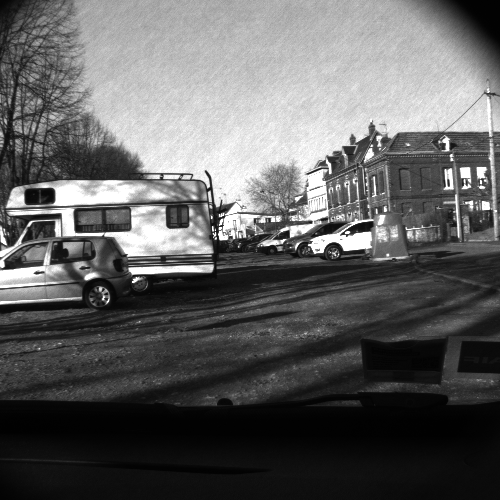
\includegraphics[width=\linewidth]{2474_I0.png}
	\end{subfigure}%
	\begin{subfigure}{0.25\textwidth}
		\centering
		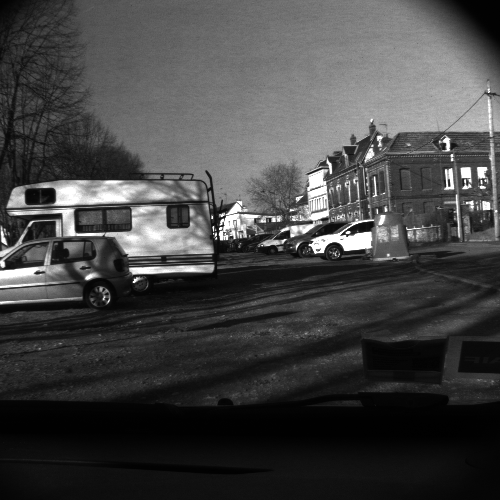
\includegraphics[width=\linewidth]{2474_I45.png}
	\end{subfigure}%
	\begin{subfigure}{0.25\textwidth}
		\centering
		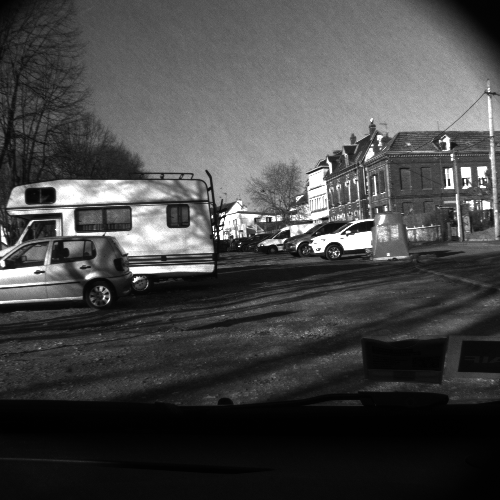
\includegraphics[width=\linewidth]{2474_I90.png}
	\end{subfigure}%
	\begin{subfigure}{0.25\textwidth}
		\centering
		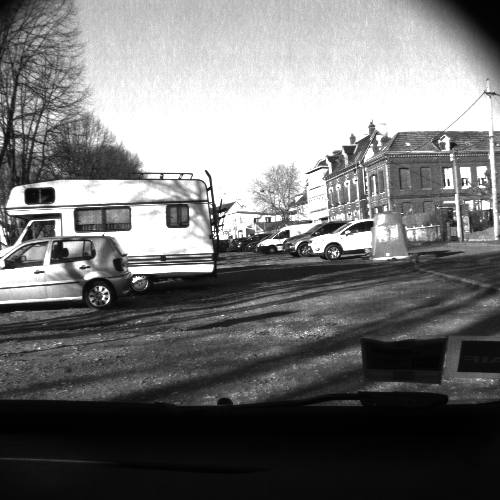
\includegraphics[width=\linewidth]{2474_I135.png}
	\end{subfigure}
	\caption[Example of a polarimetric image]{Example of a polarimetric image. From left to right, the intensities corresponding to the polarizer rotation angles 0$\degree$, 45$\degree$, 90$\degree$ and 135$\degree$.}
	\label{fig:polar_overview intensities}
\end{figure}

The linearly-polarized reflected light can be described by measurable parameters, specifically by the linear Stokes vectors. These parameters are encoded as an image $\vs \in \spaceS \subset \spaceR^{n\times p\times 3}$ such that each pixel $\vs_{i,j}$ of this image is a Stokes vector $\vs_{i,j} = \begin{bmatrix} \vs_{{i,j}_0} & \vs_{{i,j}_1} & \vs_{{i,j}_2} \end{bmatrix}^\top \in \spaceR^3$, $\forall i\leq n,  j\leq p$  . Here, $\vs_0>0$ represents the total intensity, $\vs_1$ the amount of horizontally and vertically linearly polarized light and $\vs_2$ the amount of linearly polarized light at $\pm$~45\degree. 

Associated with each polarimetry encoding format is its so-called calibration matrix $\ma$ that allows for computing the Stokes vectors. In this work, we define the calibration matrix as
%
\begin{equation}
\ma = \frac{1}{2} {\begin{bmatrix}
		1 & \cos(2\alpha_1) & \sin(2\alpha_1) \\
		1 & \cos(2\alpha_2) & \sin(2\alpha_2) \\
		1 & \cos(2\alpha_3) & \sin(2\alpha_3) \\
		1 & \cos(2\alpha_4) & \sin(2\alpha_4)
\end{bmatrix}}
\\
=  \frac{1}{2} {\begin{bmatrix}
		1 & 1 & 0 \\
		1 & 0 & 1 \\
		1 & -1 & 0 \\
		1 & 0 & -1
\end{bmatrix}} \enspace. \nonumber
\label{eq3:calibration_matrix}
\end{equation}
%
Using this calibration matrix, we define the relationship between the Stokes vectors $\vs \in \spaceR^{n\times p \times 3}$ and the light intensities $\vy \in \spaceR^{n \times p \times 4}$ reaching the camera as
%
\begin{equation}
	\vy = \ma\vs \enspace, 
	\label{eqn:IAS}
\end{equation}
%
\noindent where $\ma \in \mathbb{R}^{4\times 3}$ refers to the calibration matrix of the polarization camera. 

To compute the Stokes parameters from the measured intensities (equation \ref{eqn:IAS}), we require $\ma^\dagger = (\ma^\top \ma)^{-1} \ma^\top \in \mathbb{R}^{3\times 4}$ the pseudo-inverse (or Moore-Penrose inverse) of the matrix $\ma$. The relationship between $\vs$ and $\vy$ is defined for each pixel as

\begin{equation}
	\vs_{i,j} = \ma^\dagger \vy_{i,j} 
	\forall i\leq n, j\leq p \nonumber
	\label{eqn:stokes2} \enspace.
\end{equation}

In our work, the pseudo-inverse $\ma_\dagger$ of the calibration matrix $\ma$ is

\begin{equation}
	\ma_\dagger = 
\begin{bmatrix}
	1 & 0 & 1 & 0 \\
	1 & 0 & -1 & 0 \\
	0 & 1 & 0 & -1
\end{bmatrix}
\enspace,
\end{equation}

thus we have the relation

\begin{equation}
	\vs_{i,j} =  \ma^\dagger \vy_{i,j}  =
	\begin{bmatrix}
		1 & 0 & 1 & 0 \\
		1 & 0 & -1 & 0 \\
		0 & 1 & 0 & -1
	\end{bmatrix}
	\begin{bmatrix} 
		\vy_{{i,j}_0} \\
		\vy_{{i,j}_{45}} \\
		\vy_{{i,j}_{90}} \\
		\vy_{{i,j}_{135}}
	\end{bmatrix} 
	= 
	\begin{bmatrix} 
		\vy_{0_{i,j}} + \vy_{{i,j}_{90}} \\
		\vy_{0_{i,j}} - \vy_{{i,j}_{90}} \\
		\vy_{{i,j}_{45}} - \vy_{{i,j}_{135}} 
	\end{bmatrix}\\
	\forall i\leq n, j\leq p \nonumber \enspace .
\end{equation}

\subsection{Physical constraints of polarimetry}

A polarimetry-encoded image $\vy$ is considered to be valid if its Stokes values satisfy two main conditions: they must physically admissible and be the result of an acquisition process that use the right calibration. Since we are interested in generating new polarimetric images, they will have to comply with these essential constraints. 

To ensure that the Stokes vectors $\vs$ are physically admissible, we rely on the degree of polarization (\ac{DOP}) \citep{Ainouz2013}. The $\ac{DOP}\in [0,1]$ refers to the amount of polarized light in a wave, where a \ac{DOP} of 1  represents a totally polarized light, 0 for un-polarized light and between 0 and 1 for partially polarized light. It is defined as
%
\begin{equation}
	\ac{DOP} = \frac{\sqrt{\vs_1^2+\vs_2^2}}{\vs_0} \enspace.
\end{equation}
%
Additionally, since $\vs_0$ represents the total light intensity, it cannot be 0. Thus, to be physically admissible, a Stokes vector has to meet the conditions
%
\begin{equation}
	\vs_0 > 0
	\quad \mbox{ and } \quad 
	\vs_0^2 \geqslant \vs_1^2 + \vs_2^2 \enspace.
	\label{eqn:stokes_constraint_S0}
\end{equation}
%
Then, an additional check has to be done to ensure that a polarimetric image $\vy$  has been obtained using a given calibration matrix $\ma$.  To do so, we evaluate if the image $\vy$ can be reconstructed from the Stokes vectors computed using the the pseudo-inverse $\ma^\dagger$ of the calibration matrix. By using equations \ref{eqn:IAS} and \ref{eqn:stokes2}, we can formulate the condition  
%
\begin{equation}
\label{eq:calibration_constraint}
\vy = \ma\ma^\dagger \vy \enspace.
\end{equation}
%
Note that in the case where $\ma$ is invertible, $\ma^\dagger=\ma^{-1}$ so $\ma\ma^\dagger=Id$, thus this constraint is always enforced. In general, this constraint is satisfied if and only if $\vy \in \ker(\ma\ma^\dagger-Id)$ In the specific case where the calibration matrix $\ma$ defined in Equation \ref{eq3:calibration_matrix} is used, the solution to this constraint is 
%
\begin{equation}
\Big\{\vy = \begin{bmatrix}\vy_0 & \vy_{45} &  \vy_{90} & \vy_{135}\end{bmatrix}^\top\Big| \vy_0 + \vy_{90} = \vy_{45} + \vy_{135} \Big\} \enspace.
\end{equation}
%
The proof of this result is found in appendix \ref{app:physical_prop}. 

We finally obtain a set of three polarimetric constraints $\mathcal{C}_1$, $\mathcal{C}_2$ and $\mathcal{C}_3$ formulated as 
%
\begin{eqnarray}
	\label{eq3:constraints}
	\mathcal{C}_1 &:&\vy = \ma\ma^\dagger\vy, \\
	\mathcal{C}_2 &:& \vs_0^2 \geqslant \vs_1^2 +\vs_2^2 \enspace, \nonumber\\
	\mathcal{C}_3 &:& \vs_0 > 0 \enspace. \nonumber
\end{eqnarray}

In this chapter, we consider images that satisfy this set of constraints to be physically admissible.

%%%%%%%%%%%%%%%%%%%%%%%%%%%%%%%%%%%
%%%%%%%%%%%%%%%%%%%%%%%%%%%%%%%%%%%%%%%%%%%%%%%%%%%%

\section{Unsupervised color to polarimetric image translation}
\label{sec3:related_works}

In this section, we propose a formulation of the polarimetric image generation as a constrained domain-transfer problem. We examine the limits  of the classical domain-transfer approaches and propose an overview of some recent methods that overcome these limits. 

\subsection{Polarimetric image generation as a constrained conditional image generation problem}

The problematic studied in this chapter is learning a model for generating physically realistic polarimetry-encoded images from color images in an unpaired and unsupervised way. A polarimetric image generated that way should remain semantically consistent with the input color image, i.e that it should represent the same scene and objects but in a different modality.

Thus, there are two important aspects to this problem. First, we aim to learn a generative model $\G_{XY}$  such that, for an \ac{RGB} image $\vx \in \spaceX$ issued from the distribution $\p{X}$, the generated images $\G_{XY}(\vx) = \Hat{\vy} \in \spaceY$ is issued from $\p{Y}$ the distribution of the real polarimetric images. Hence, the generated images $\Hat{\vy}$ and  their Stokes vectors $\Hat{\vs} = \ma^\dagger\Hat{\vy}$ must respect the constraints $\mathcal{C}_1$, $\mathcal{C}_2$ and $\mathcal{C}_3$ (see \ref{eq3:constraints}).

We can formulate this as
%
\begin{eqnarray}
	\label{eq:polar_constr_formulation}
	\max_{\G_{XY}}& L(\G_{XY}) = \mathop{\mathbb{E}}_{\vx\sim \p{X}} \Big[\log (\p{Y}(\G_{XY}(\vx))\Big]  \\
	\text{s.c.} & \vy_i = \ma\vs_i \enspace;\enspace \vs_{0_i}^2 \geq \vs_{1_i}^2 +\vs_{2_i}^2  \enspace\text{and}\enspace  \vs_{0_i}^2 > 0   \nonumber \\
	\text{with}  & \vs_{i} = \ma^\dagger(\G_{XY}(\vy_{i})) \quad \forall i \nonumber
\end{eqnarray}

Then, we aim to enforce the semantic consistency between the input $\vx$ and the generated image $\Hat{\vy}$. One additional requirement is that the model should be trainable in an unpaired and unsupervised way. This implies that the only available datasets consist in unpaired and unlabeled samples $\setX = \{\vx_1, ..., \vx_s\}, \vx_i \in \spaceX$ and $\setY = \{\vy_1, ..., \vy_s\}, \vy_i \in \spaceY$ from the two domains $\spaceX $ and $\spaceY$. This requirement can be approached using unsupervised domain-transfer methods.

\subsection{Approaches for unsupervised conditional domain-transfer}

In Section \ref{subs:domain_transfer}, we reviewed different approaches for unsupervised domain-transfer. Most notably, we introduced the cycle-consistency losses used in models such as \ac{CycleGAN} \citep{Zhu2017a}. These approaches consists in training two conditional \ac{GAN} models, $\G_{XY}: \spaceX \rightarrow \spaceY$ and $\G_{YX}: \spaceY \rightarrow \spaceX$, that maps samples between the distributions$\p{X}$ and $\p{Y}$ of the two domains, then training them with both the classical \ac{GAN} losses and the cycle-consistency loss, formulated as 
%
$$\esp{\vx\sim\p{\vx}} ||\vx - \Gyx(\Gxy(\vx))||_1 + \esp{y\sim\p{\vy}} ||\vy - \Gxy(\Gyx(\vy))||_1 \enspace .$$
%
The full \ac{CycleGAN}  problem can be summed up as 
%
\begin{align}
	\min_{\Gxy, \Gyx}\max_{\Dx, \Dy} & \lcycgan  (\G_{XY}, \G_{YX}, \D_X, \D_Y) = \nonumber \\ 
	\min_{\Gxy, \Gyx}\max_{\Dx, \Dy}  &\esp{\vx\sim\p{\vx}}   \Big[(1-\D_X(\vx)^2) + (\D_Y(\G_{XY}(\vx)))^2 \Big] + \esp{y\sim\p{\vy}}  \Big[(1-\D_Y(\vy))^2 + (\D_X(\Gyx(\vy)))^2 \Big] \nonumber \\
	& +\lambda \Big[ \esp{\vx\sim\p{\vx}} ||\vx - \Gyx(\Gxy(\vx))||_1 + \esp{y\sim\p{\vy}} ||\vy - \Gxy(\Gyx(\vy))||_1 \Big] \nonumber\enspace .
\end{align}
%
While these approaches allow for efficient domain-translation (and notably image-to-image translation), they do not integrate domain-specific knowledge, for example the polarimetric constraints mentioned in Section \ref{sec3:physical_prop}.

To constrain the domain-transfer process, several approaches rely on adding a task specific loss to the \ac{CycleGAN} objective. This can be done in a supervised way, leveraging on labeled data by training a task model and minimizing its error, or in an unsupervised way with an explicit task loss.

\textbf{TD-GAN} \citep{Zhang2018c} integrates a conditioning process in a task of semantic segmentation from organ X-ray images. To do so, the authors rely on existing labeled datasets of digitally reconstructed radiographs (DRRs), which they to train a semantic segmentation model. They use this model to condition a \ac{CycleGAN}-like model that translates images from the X-ray to the DRR domain by adding the segmentation loss to the \ac{CycleGAN} objective. In other words, DRR images are translated to X-ray, then back to DRRs, segmented using the pre-trained model and then compared to the ground truth segmentation using binary cross-entropy. 

\textbf{CyCADA} \citep{Hoffman2018} also implements the idea of using pre-trained classifiers or segmentation models to condition domain-transfer.  They achieve this conditioning by comparing the classes (or segmentation maps) of the source and generated images, then adding the loss of these models to the objective of a \ac{CycleGAN}-like model. While this conditioning process requires a pre-trained model, it does not require for the datasets to be labeled. They demonstrate this approach for domain-transfer with datasets such as \ac{MNIST} \citep{LeCun1998a} and Street View House Numbers(SVHN) \citep{Netzer2011} for a digit classification task, and the SYNTHIA \citep{Ros2016}, GTA \citep{Richter2016} and Cityscapes \citep{Cordts2015} datasets for road scenes semantic segmentation.

Several methods also leverage on this conditioning approach to enhance the performance of the domain-transfer task. \textbf{VIGAN} \citep{Shang2017} includes a denoising auto-encoder; the aforementioned \textbf{CyCADA} an adversarial loss on the features extracted by a pre-trained classifier; \textbf{Attention-GAN} \citep{Chen2018b} uses an attention mechanism.



\section{Generating polarimetric images with auxiliary tasks for domain-transfer modeling}
\label{sec3:solutions}

The problem studied in this chapter is image-to-image translation from \ac{RGB} images to the polarimetric domain. In the previous sections, we formalized the constraints of polarimetric imaging and reviewed the different approaches for image-to-image translation based on generative modeling, as well as conditioning mechanism based on task-specific losses.

As  a main contribution in this chapter, we propose here three variants of the \ac{CycleGAN} approach for conditioning the domain translation task with the constraints of polarimetry. Our first approach is to formulate a relaxation of both the calibration constraint (see Equation \ref{eq:calibration_constraint}) and the constraint of physical admissibility (see Equation \ref{eq:polar_constr_formulation}) and add the obtain costs to the \ac{CycleGAN} losses. For the second approach, we formulate a projection operator for the constraint of physical admissibility, train the network with the relaxed calibration constraint and use this operator to project the generated images in the space of the constraints. Finally for the third approach, we formulate a distance between the generated sample and its projection and we add it to the \ac{CycleGAN} objective.

We evaluate these methods on a road-scene \ac{RGB} to polarimetric image translation. We compare the visual quality of the samples and the respect of the polarimetric constraints. We further examine the physical admissibility of the generated images by studying the impact of using our approaches as a data-augmentation technique for a road-scene detection task. \CR{We observe that our approaches outperforms the unconstrained \ac{CycleGAN} on every aspects and that using generated polarimetric images contributes to enhance the performances on the road-scene detection task.}

\subsection{Auxiliary tasks for color to polarimetric images domain-transfer}

As discussed above, our main goal is to learn a generative model able to produce realistic polarization-based images starting from \ac{RGB} images. To generate a polarimetric image  from an \ac{RGB} image, we propose to use the CycleGAN approach to learn the translation models $\G_{XY}$ between $\spaceX$ the space of the polarimetric images and $\spaceY$ the RGB image domain. Let $\Hat{\vy} \in \spaceR^{n \times m \times 4}$ be a generated polarimetric image. To be physically admissible, it has to satisfy the admissibility constraints (\ref{eqn:stokes_constraint_S0}) and the calibration constraint (\ref{eq:calibration_constraint}). 

\subsubsection{- Relaxation of the constraints}

\begin{figure} 
	\centering
	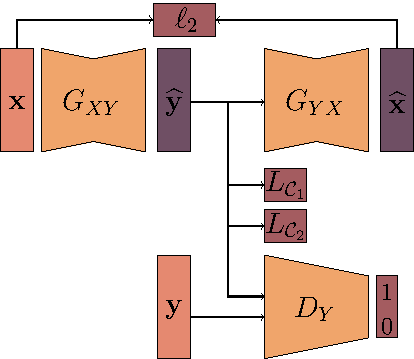
\includegraphics[width=\textwidth*2/3]{ours_const}
	\caption{Overview of the CycleGAN training process extended with $L_{\mathcal{C}_1}$ and $L_{\mathcal{C}_2}$.}
	\label{fig:overview_polarCycle}
\end{figure}

By design, the first component of the Stokes vector is always positive as it represents the total intensity reflected from an object.  As the last layer of the generation models customary uses the hyperbolic tangent as activation function, each output intensity $\Hat{\vy}$ is within the range $]-1,1[$ which we scale to $]0,255[$. Hence $\hat{\vs}_0=\hat{\vy}_0+\hat{\vy}_{90}$ (see equation (\ref{eqn:stokes2})) is ensured to be strictly positive. Therefore, constraint $\mathcal{C}_3$ can be deemed satisfied for the real and the generated polarimetric images. To handle the remaining constraints $\mathcal{C}_1$ and $\mathcal{C}_2$, one could resort to the Lagrangian dual of CycleGAN optimization problem (\ref{eq:cyclegan}) subject to these constraints. However, this may be computationally expensive, as it requires to entirely optimize four neural networks (respectively the discrimination and the mapping network models) in an inner loop of a dual ascent algorithm. Moreover the overall optimization procedure may not be stable because of the min-max game involved in the CycleGAN learning. In order to derive  an efficient algorithm to learn CycleGAN under output constraints, we introduce a relaxation of the problem. Instead of strictly enforcing the constraints, as in \citeq{eq:polar_constr_formulation}, we measure how far the generated image pixels are from the feasibility domain through additional cost functions we attempt to minimize.
%
For the constraint $\mathcal{C}_1$, a $\ell_2$ distance between the generated image $G_{YX}$ and $\ma\Hat{\vs}$ is proposed. It reads
%
\begin{equation}
L_{\mathcal{C}_1} (\G_{XY}) = \mathop{\mathbb{E}}_{\vx\sim \p{X}} ||\G_{XY}(\vx) - \ma\ma^\dagger\G_{XY}(\vx)||_2\enspace, 
\label{eqn:ls}
\end{equation}
%
Similarly, to enforce the constraint $\mathcal{C}_2$, a rectified linear penalty $L_{\mathcal{C}_2}$ is considered. It is defined by:
%
\begin{equation}
L_{\mathcal{C}_2} (\G_{XY}) = \mathop{\mathbb{E}}_{\vx\sim \p{X}}  \max\left(\Hat{\vs}_1^2 + \Hat{\vs}_2^2 -
\Hat{\vs}_0^2, 0 \right)\enspace,
\label{eqn:lreg}
\end{equation}
%
with $\hat{\vs} = \begin{bmatrix}	\Hat{\vs_0} & 	\Hat{\vs_1} & 	\Hat{\vs_2} \end{bmatrix}^\top = \ma^\dagger\G_{XY}(\vx)$.

The loss $L_{\mathcal{C}_1}$ translates the respect of the acquisition conditions according to the calibration matrix $A$ while  $L_{\mathcal{C}_2}$ is related to the physical admissibility constraint on the deduced Stokes vectors from the generated image.


\begin{algorithm}[!t]
	\begin{algorithmic}[]
		\REQUIRE{$\trainsetX$ and $\trainsetY$ two unpaired datasets, $\Gxy$ and $\Gyx$ the mapping networks, $\Dx$ and $\Dy$ the discrimination models, $m$ the mini-batch size, $\ma$ the calibration matrix and $\ma^\dagger$ its pseudo-inverse, $\lambda, \mu, \nu$ hyperparameters}
		\REPEAT
		\STATE sample a mini-batch $\lbrace \vx_i \rbrace_{i=1}^m$ from $\trainsetX$\;
		\STATE sample a mini-batch $\lbrace \vy_i \rbrace_{i=1}^m$ from $\trainsetY$\;
		\STATE update $\Dx$ by stochastic gradient descent of
		\STATE \ \ \ \ $ \sum_{i=1}^{m}\big(\Dx(\vx_i)-1)^2 + (\Dx(\Gyx(\vy_i))\big)^2$
		\STATE update $\Dy$ by stochastic gradient descent of
		\STATE \ \ \ \ $ \sum_{i=1}^{m}\big(\Dy(\vy_i)-1)^2 + (\Dy(\Gxy(\vx_i))\big)^2$
		\STATE sample a mini-batch $\lbrace \vx_i \rbrace_{i=1}^m$ from $\trainsetX$\;
		\STATE sample a mini-batch $\lbrace \vy_i \rbrace_{i=1}^m$ from $\trainsetY$\;
		\STATE for $i=1$ to $n$, compute $\hat{\vs_i} = \begin{bmatrix}	\Hat{\vs_{0_i}} & 	\Hat{\vs_{1_i}} & 	\Hat{\vs_{2_i}}\end{bmatrix}^\top = \ma^\dagger\G_{XY}(\vx_i)$.
		\STATE update $\Gxy$ by stochastic gradient descent of
		\STATE \ \ \ \ $ \sum_{i=1}^n\big(\Dy(\Gxy(\vx_i))-1\big)^2 + \lambda \big(||\vx_i - \Gyx(\Gxy(\vx_i)\big)||_1 +||\vy_i -\Gxy(\Gyx(\vy_i))||_1\big)$
		\STATE \ \ \ \ \ \ $+ \mu \big(\ma\Hat{\ma^\dagger\G_{XY}(\vx_i)}\Big)+ \nu \big(\max(\vs_{1_i}^2 + \vs_{2_i}^2 - \vs_{0_i}^2, 0\big)$
		\STATE update $\Gyx$ by stochastic gradient descent of
		\STATE \ \ \ \ $ \sum_{i=1}^n \big(\Dx(\Gyx(\vy_i))-1\big)^2+ \lambda \big(||\vx_i - \Gyx(\Gxy(\vx_i))||_1 + ||\vy_i - \Gxy(\Gyx(\vy_i))||_1\big)$\;
		\UNTIL a stopping condition is met
	\end{algorithmic}
	\caption{CycleGAN with relaxed constraints training algorithm}
	\label{alg:cyclegan_relaxed_train}
\end{algorithm}


Gathering all these elements, we train our CycleGAN under physical constraints, by optimizing the following objective function:
%
\begin{equation}
L_{final}(\G_{XY}, \G_{YX}, \D_X, \D_Y)= L_{CycleGAN}(\G_{XY}, \G_{YX}, \D_X, \D_Y)+\mu L_{\mathcal{C}_1}(\G_{XY}) + \nu L_{\mathcal{C}_2}(\G_{XY}) \enspace.
\label{eqn:lfinal}
\end{equation}
%
The non-negative hyper-parameters $\mu$ and $\nu \in \mathbb{R}^{+}$ control respectively the balance of admissibility and calibration constraints according to the CycleGAN loss $L_{CycleGAN}$ (see equation~\eqref{eq:cyclegan}). As the values of $L_{\mathcal{C}_1}$ and $L_{\mathcal{C}_2}$ are computed pixel-wisely, we consider their averages over the whole image in the objective function. The training principle of the proposed generative model is illustrated in Figure~\ref{fig:overview_polarCycle} and detailed in Algorithm~\ref{alg:cyclegan_relaxed_train}.

\subsubsection{- Proximal method}

	We aim to generate images $ \Hat{\vy} =  \G_{XY}(\vx)$, where $\vx \in \spaceX$ is a sample from the \ac{RGB} domain, such that $\Hat{\vs} = \ma^\dagger\Hat{\vy} \in  \spaceS$ the space of the Stokes vectors. Each of the vectors must  respect $\mathcal{C}_1$, $\mathcal{C}_2$ and $\mathcal{C}_3$, which correspond to a second-order cone, or Lorentz cone \citep{Boyd2004}. Thus, let
%
	\begin{equation}
		\setC = \left \lbrace (\vs_0,\vs_{1,2}) \in  \spaceS \,\, \Big| \,\, \|\vs_{1,2}\|_2 \leq \vs_0, \,\, \vs_{1,2} = \begin{bmatrix} \vs_1 \\ \vs_2 \end{bmatrix} \right \rbrace \enspace,
	\end{equation}
 %	
 \begin{algorithm}[!t]
 	\begin{algorithmic}[]
 		\REQUIRE{$\trainsetX$ and $\trainsetY$ two unpaired datasets, $\Gxy$ and $\Gyx$ the mapping networks, $\Dx$ and $\Dy$ the discrimination models, $m$ the mini-batch size, $\ma$ the calibration matrix and $\ma^\dagger$ its pseudo-inverse, $\lambda, \mu$ hyperparameters}
 		\REPEAT
 		\STATE sample a mini-batch $\lbrace \vx_i \rbrace_{i=1}^m$ from $\trainsetX$\;
 		\STATE sample a mini-batch $\lbrace \vy_i \rbrace_{i=1}^m$ from $\trainsetY$\;
 		\STATE update $\Dx$ by stochastic gradient descent of
 		\STATE \ \ \ \ $ \sum_{i=1}^{m}\big(\Dx(\vx_i)-1)^2 + (\Dx(\Gyx(\vy_i))\big)^2$
 		\STATE update $\Dy$ by stochastic gradient descent of
 		\STATE \ \ \ \ $ \sum_{i=1}^{m}\big(\Dy(\vy_i)-1)^2 + (\Dy(\ma\Pi_{\setC}(\ma^\dagger\Gxy(\vx_i)))\big)^2$
 		\STATE sample a mini-batch $\lbrace \vx_i \rbrace_{i=1}^m$ from $\trainsetX$\;
 		\STATE sample a mini-batch $\lbrace \vy_i \rbrace_{i=1}^m$ from $\trainsetY$\;
 		\STATE update $\Gxy$ by stochastic gradient descent of
 		\STATE \ \ \ \ $ \sum_{i=1}^n\big(\Dy(\Gxy(\vx_i))-1\big)^2$ $+ \mu \big(\ma\ma^\dagger\G_{XY}(\vx_i)\Big)$
 		\STATE \ \ \ \ \ \ $ + \lambda \big(||\vx_i - \Gyx(\ma\Pi_{\setC}(\ma^\dagger\Gxy(\vx_i))\big)||_1 +||\vy_i -\ma\Pi_{\setC}(\ma^\dagger\Gxy(\Gyx(\vy_i)))||_1\big)$
 		\STATE update $\Gyx$ by stochastic gradient descent of
 		\STATE \ \ \ \ $ \sum_{i=1}^n \big(\Dx(\Gyx(\vy_i))-1\big)^2 $
 		\STATE \ \ \ \ \ \ 	$+ \lambda \big(||\vx_i - \Gyx(\ma\Pi_{\setC}(\ma^\dagger\Gxy(\vx_i)))||_1 + ||\vy_i -\ma\Pi_{\setC}(\ma^\dagger\Gxy(\Gyx(\vy_i))||_1\big)$\;
 		\UNTIL a stopping condition is met
 	\end{algorithmic}
 	\caption{Training algorithm for CycleGAN with projected images}
 	\label{alg:cyclegan_train_projection}
 \end{algorithm}

\begin{figure} 
	\centering
	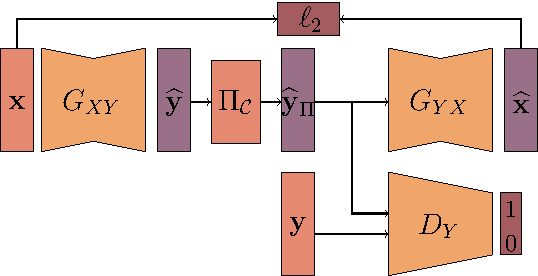
\includegraphics[width=\textwidth]{ours_proj}
	\caption{Overview of the CycleGAN training process with extended the projection operator. The $L_{\setC_1}$ is omitted.}
	\label{fig:overview_polarCycle_proj}
\end{figure}

 	a convex set whose vectors satisfy the aforementioned constraints. As such, we can reformulate the problem \citeq{eq:polar_constr_formulation} as
 %	
 	\begin{eqnarray}
 		\label{eq:polar_set_formulation}
 		\max_G& L(G) = \mathop{\mathbb{E}}_{\vx\sim \p{X}} \Big[\log (\p{Y}(\G_{XY}(\vx))\Big]  \\
 		\text{s.c.}  & \ma^\dagger(\G_{XY}(\vx_{i})) \in \setC, \forall i \nonumber \enspace .
 	\end{eqnarray}
% 	
With such a membership constraint, the projection operator $\Pi_{\setC}$ on $\setC$ can be defined as finding the solution to the optimization problem
%	
	\begin{equation}
		\label{eq:projection_op}
		\min_{(\vr, \vu) \in \setC} \frac{1}{2} \| (\vs_0, \vs_{1,2}) - (\vr, \vu)\|_2^2 \enspace,
	\end{equation}
%
	which has a closed-form solution \citep{Parikh2014} as
%	
	\begin{equation}
		\label{eq:proj_lorentz_cone_2}
		\Pi_{\setC}(\vs_0, \vs_{1,2}) = \left \lbrace
		\begin{array}{lll}
			(\vs_0, \vs_{1,2}) & \text{if} & \| \vs_{1,2} \|_2 \leq \vs_0 \\
			\frac{1+ \vt/\|\vs_{1,2}\|_2}{2} (\|\vs_{1,2}\|_2, \vs_{1,2}) & \text{if} & \| \vs_{1,2} \|_2 > \vs_0
		\end{array}
		\right.
	\end{equation}
%
We can introduce this projection operator to the training algorithm instead of the loss term obtain by the relaxation of $\setC_2$.  To do so, the output of $\G_{XY}$ is systematically projected onto $\setC$ using $\Pi_{\setC}$ as
%
\begin{equation}
	\Hat{\vy}_{\Pi_{\setC}} = \ma\Pi_{\setC}(\ma^\dagger\G_{XY(\vx)}) \enspace,
\end{equation} 
%
with $\vx \in \spaceX$ an \ac{RGB} image. This process is summed up in Algorithm \ref{alg:cyclegan_train_projection} and illustrated in Figure \ref{fig:overview_polarCycle_proj}.

\begin{algorithm}[!t]
	\begin{algorithmic}[]
		\REQUIRE{$\trainsetX$ and $\trainsetY$ two unpaired datasets, $\Gxy$ and $\Gyx$ the mapping networks, $\Dx$ and $\Dy$ the discrimination models, $m$ the mini-batch size, $\ma$ the calibration matrix and $\ma^\dagger$ its pseudo-inverse, $\lambda, \mu, \nu$ hyperparameters}
		\REPEAT
		\STATE sample a mini-batch $\lbrace \vx_i \rbrace_{i=1}^m$ from $\trainsetX$\;
		\STATE sample a mini-batch $\lbrace \vy_i \rbrace_{i=1}^m$ from $\trainsetY$\;
		\STATE update $\Dx$ by stochastic gradient descent of
		\STATE \ \ \ \ $ \sum_{i=1}^{m}\big(\Dx(\vx_i)-1)^2 + (\Dx(\Gyx(\vy_i))\big)^2$
		\STATE update $\Dy$ by stochastic gradient descent of
		\STATE \ \ \ \ $ \sum_{i=1}^{m}\big(\Dy(\vy_i)-1)^2 + (\Dy(\Gxy(\vx_i))\big)^2$
		\STATE sample a mini-batch $\lbrace \vx_i \rbrace_{i=1}^m$ from $\trainsetX$\;
		\STATE sample a mini-batch $\lbrace \vy_i \rbrace_{i=1}^m$ from $\trainsetY$\;
		\STATE for $i=1$ to $n$, compute $\hat{\vs_i} = \begin{bmatrix}	\Hat{\vs_{0_i}} & 	\Hat{\vs_{1_i}} & 	\Hat{\vs_{2_i}}\end{bmatrix}^\top = \ma^\dagger\G_{XY}(\vx_i)$.
		\STATE update $\Gxy$ by stochastic gradient descent of
		\STATE \ \ \ \ $ \sum_{i=1}^n\big(\Dy(\Gxy(\vx_i))-1\big)^2 + \lambda \big(||\vx_i - \Gyx(\Gxy(\vx_i)\big)||_1 +||\vy_i -\Gxy(\Gyx(\vy_i))||_1\big)$
		\STATE \ \ \ \ \ \ $+ \mu \big(\ma\Hat{\ma^\dagger\G_{XY}(\vx_i)}\Big)+ \nu \|\ma^\dagger \G_{XY}(\vx_i) - \Pi_\setC(\ma^\dagger \G_{XY}(\vx_i))\|^2$\;
		\STATE update $\Gyx$ by stochastic gradient descent of
		\STATE \ \ \ \ $ \sum_{i=1}^n \big(\Dx(\Gyx(\vy_i))-1\big)^2+ \lambda \big(||\vx_i - \Gyx(\Gxy(\vx_i))||_1 + ||\vy_i - \Gxy(\Gyx(\vy_i))||_1\big)$\;
		\UNTIL a stopping condition is met
	\end{algorithmic}
	\caption{CycleGAN with proximal training algorithm}
	\label{alg:cyclegan_train_proximal}
\end{algorithm}

\begin{figure} 
	\centering
	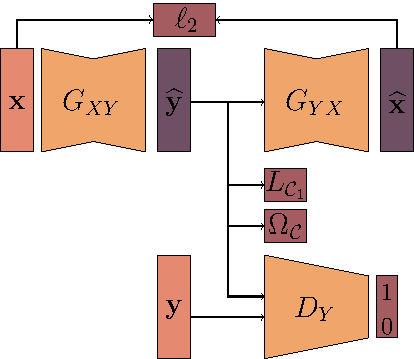
\includegraphics[width=\textwidth*2/3]{ours_prox}
	\caption{Overview of the CycleGAN training process extended with the $L_{\setC_1}$ and proximal losses}
	\label{fig:overview_polarCycle_prox}
\end{figure}

	Another solution is to formulate an alternative version to the loss induced by relaxation (\ref{eqn:lreg}) that measures the distance between the Stokes vectors of the generated image and their projection on the constraint space, as
%	
	\begin{equation}
		\label{eq:polar_proximal_formulation}
		L_{prox} (\G_{XY}) = \mathop{\mathbb{E}}_{\vx\sim \p{X}} \Big[\|\ma^\dagger \G_{XY}(\vy) - \Pi_\setC(\ma^\dagger \G_{XY}(\vy))\|^2\Big] \enspace  ,
	\end{equation}
%	
	with $\lambda$ a regularization parameter. This loss can then be added to the \ac{CycleGAN} approach, in the same fashion as the relaxed loss. This process is summed up in Algorithm \ref{alg:cyclegan_train_proximal} and illustrated in Figure \ref{fig:overview_polarCycle_prox}. Note that the gradient of the distance $\Omega_\setC = \|A^\dagger \G_{XY}(\vy) - \Pi_\setC(A^\dagger \G_{XY}(\vy))\|^2$ can be expressed as 
%
	\begin{equation}
		\nabla_{\G_{XY}} \Omega_{\setC}(\vs) = \left( \vs - \Pi_{\setC}(\vs) \right) \times \left \lbrace
		\begin{array}{lll}
			0 & \text{if} & \|\vs_{1,2}\|_2 \leq \vs_0 \\
			\nabla_{\G_{XY}} \vs - \nabla_{\G_{XY}}   \frac{1}{2} \big[(1+ \frac{\vs_0}{\|\vs_{1,2}\|_2}) (\|\vs_{1,2}\|_2, \vs_{1,2})\big]  & \text{if} & \|\vs_{1,2} \|_2 > \vs_0
		\end{array}
		\right.
		\label{eq:grad_lorentz_cone_3}
	\end{equation}
%
	Such an approach for learning models with constraints has been used, for example, by \citet{Kervadec2019} as an alternative to the Lagrangian version of ai image segmentation problem under volume constrains, determined by a convolutional neural network \citep{Pathak2015}.



\subsection{Experimental evaluation}
\label{sec3:experiments}

Hereafter, the experimental setup, including the image generation procedure and its evaluation, is presented. 

\subsubsection{-  Polarimetric images generation using CycleGAN- based approaches} \label{subsec:polar_gen}

To conduct the experiments, we rely on the polarimetric dataset presented in \citep{Blin2020} whose details are summarized in Table \ref{tab:dataset_properties}. From this dataset we select 2485 unpaired images from each domain (RGB and polarimetry). Example instances are shown in Figures~\ref{fig:polar_example} and~\ref{fig:rgb_example}  for polarimetric and RGB images respectively. The polarimetric images are of dimension $500 \times 500 \times 4$. The latter dimension is due to the four intensities acquired by the camera, namely $\vy_0, \vy_{45}, \vy_{90}$ and $\vy_{135}$. The RGB images are of dimension $906 \times 945 \times 3$.
\begin{figure}[t]
	\centering
	\begin{subfigure}{.2\textwidth}
		\centering
		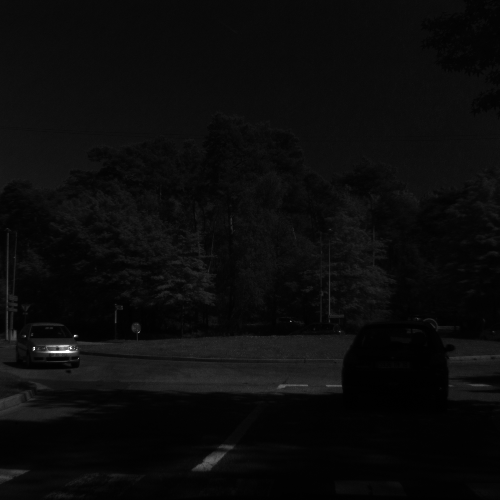
\includegraphics[width=\linewidth]{1625_I0.png}
	\end{subfigure}%
	\begin{subfigure}{.2\textwidth}
		\centering
		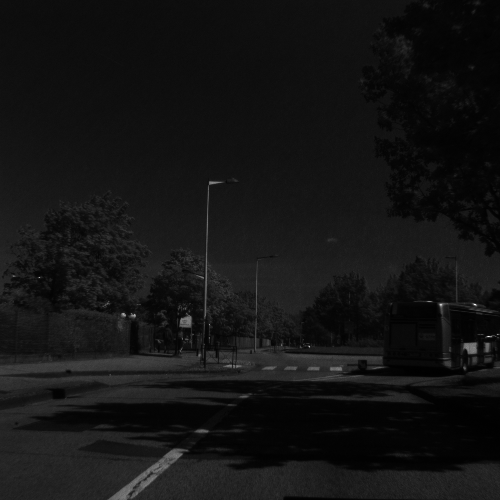
\includegraphics[width=\linewidth]{240_I0.png}
	\end{subfigure}%
	\begin{subfigure}{.2\textwidth}
		\centering
		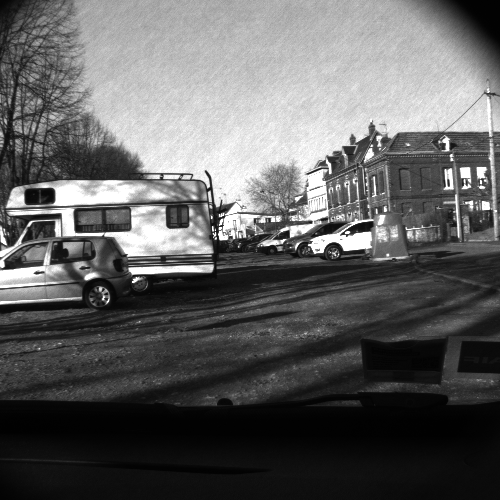
\includegraphics[width=\linewidth]{2474_I0.png}
	\end{subfigure}%
	\begin{subfigure}{.2\textwidth}
		\centering
		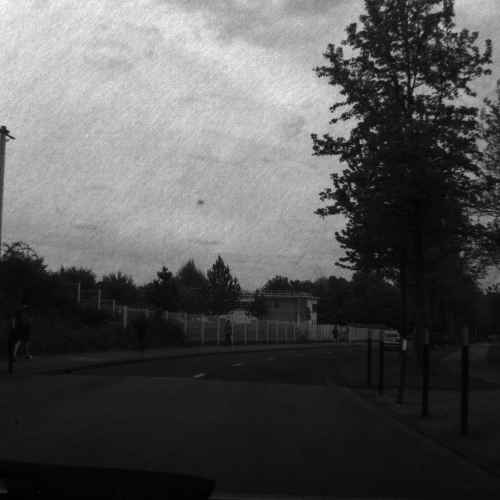
\includegraphics[width=\linewidth]{48_I0.png}
	\end{subfigure}%
	\begin{subfigure}{.2\textwidth}
		\centering
		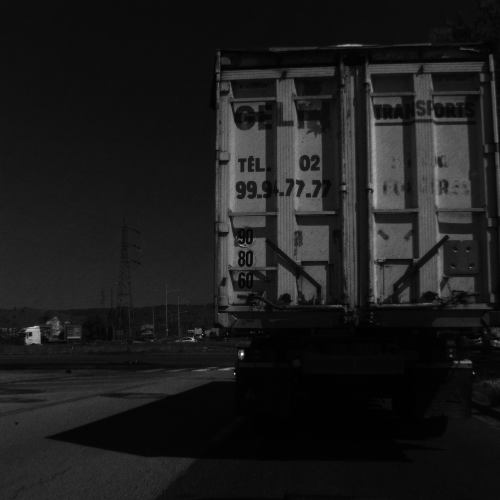
\includegraphics[width=\linewidth]{766_I0.png}
	\end{subfigure}
	\caption[Examples of images in the polarimetric dataset ]{Examples of images in the polarimetric dataset \citep{Blin2020}. Only the intensities $I_0$ are shown here.}
	\label{fig:polar_example}
\end{figure}

\begin{table}
	\begin{center}
		\begin{tabular}{c c c c c}
			\Bigrule
			Class & Train & Val & Test \\
			\bigrule
			Images & 3861 & 1248 & 509 \\
			\bigrule
			car & 19587 & 3793 & 2793 \\
			person & 2049 & 294 & 161 \\
			bike & 16 & 35 & 3 \\
			motorbike & 52 & 4 & 5 \\
		\end{tabular}
		\caption[Polarimetric dataset features]{Polarimetric dataset features. The bottom rows indicate the total number of instances within each class.}
		\label{tab:dataset_properties}
	\end{center}
\end{table}


\begin{figure}
	\centering
	\begin{subfigure}{.2\textwidth}
		\centering
		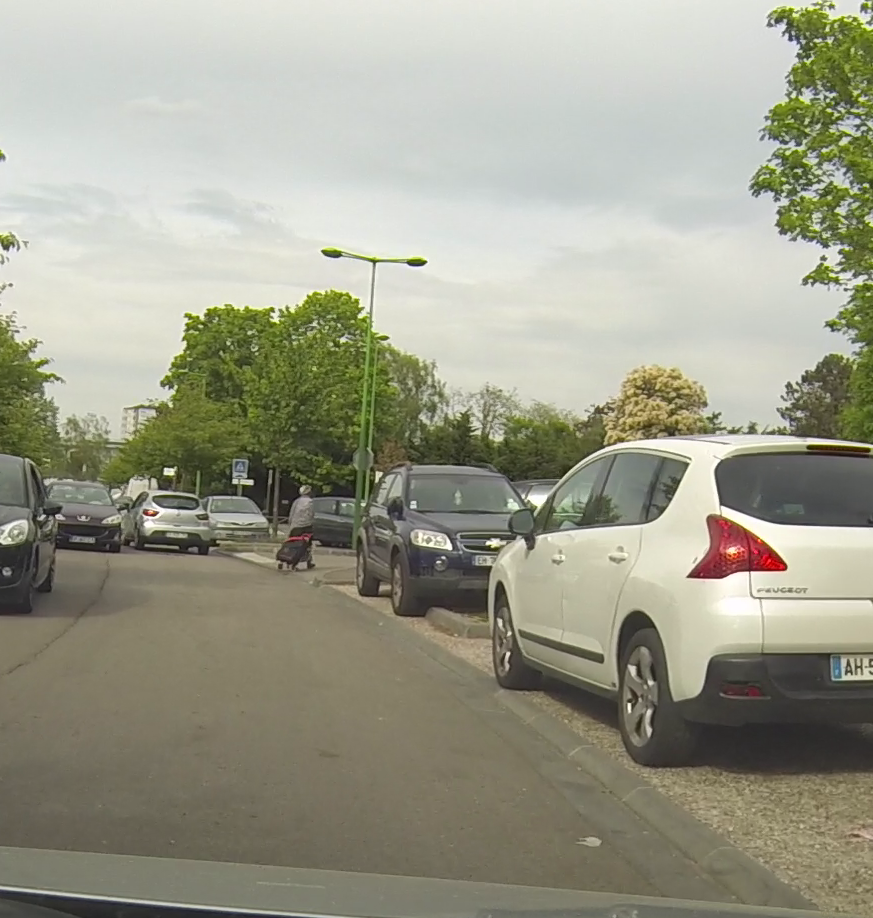
\includegraphics[width=\linewidth]{0030144.png}
	\end{subfigure}%
	\begin{subfigure}{.2\textwidth}
		\centering
		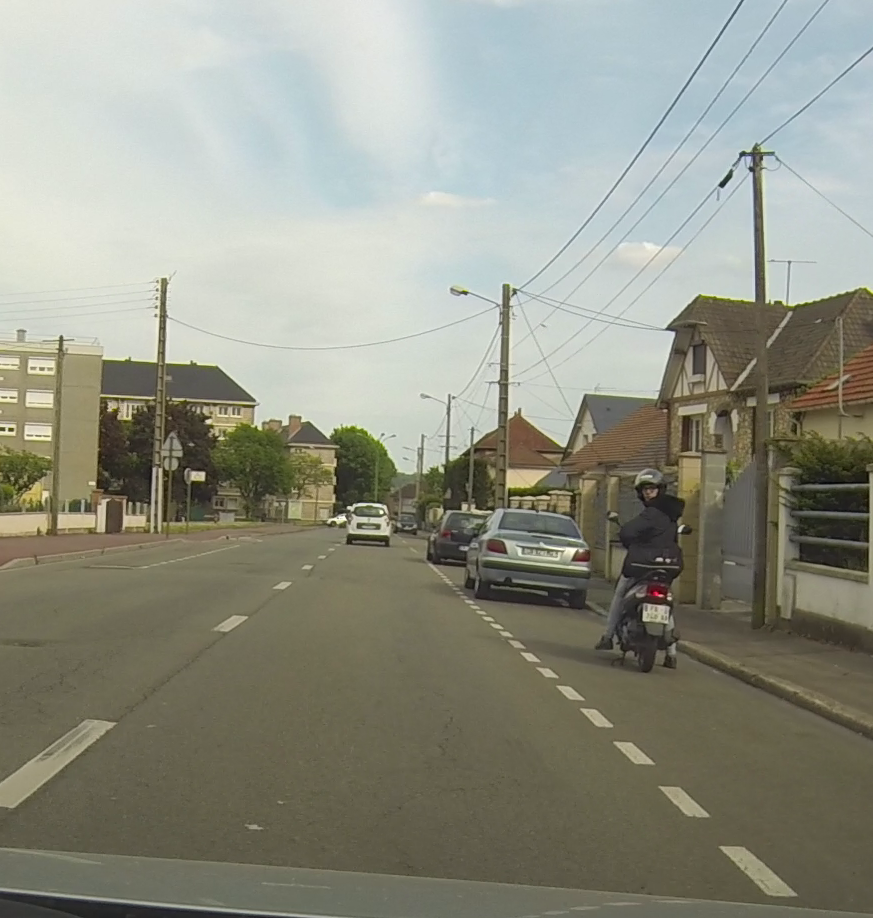
\includegraphics[width=\linewidth]{0038544.png}
	\end{subfigure}%
	\begin{subfigure}{.2\textwidth}
		\centering
		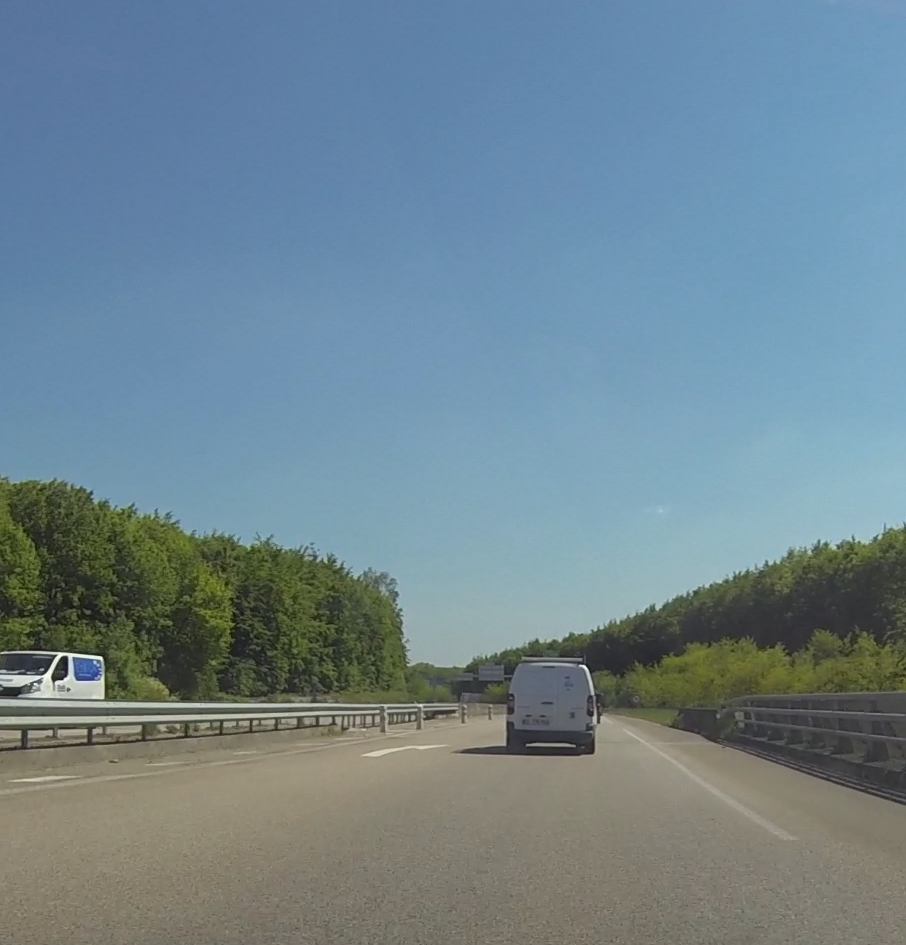
\includegraphics[width=\linewidth]{0025879.png}
	\end{subfigure}%
	\begin{subfigure}{.2\textwidth}
		\centering
		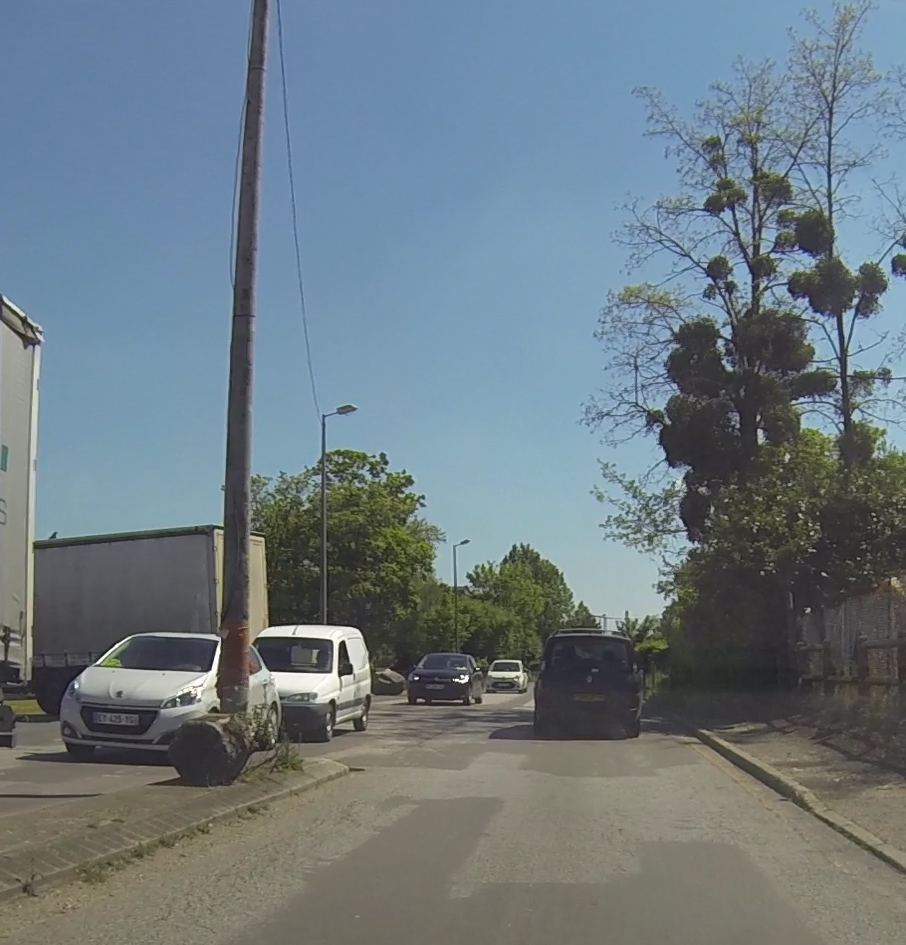
\includegraphics[width=\linewidth]{0032059.png}
	\end{subfigure}%
	\begin{subfigure}{.2\textwidth}
		\centering
		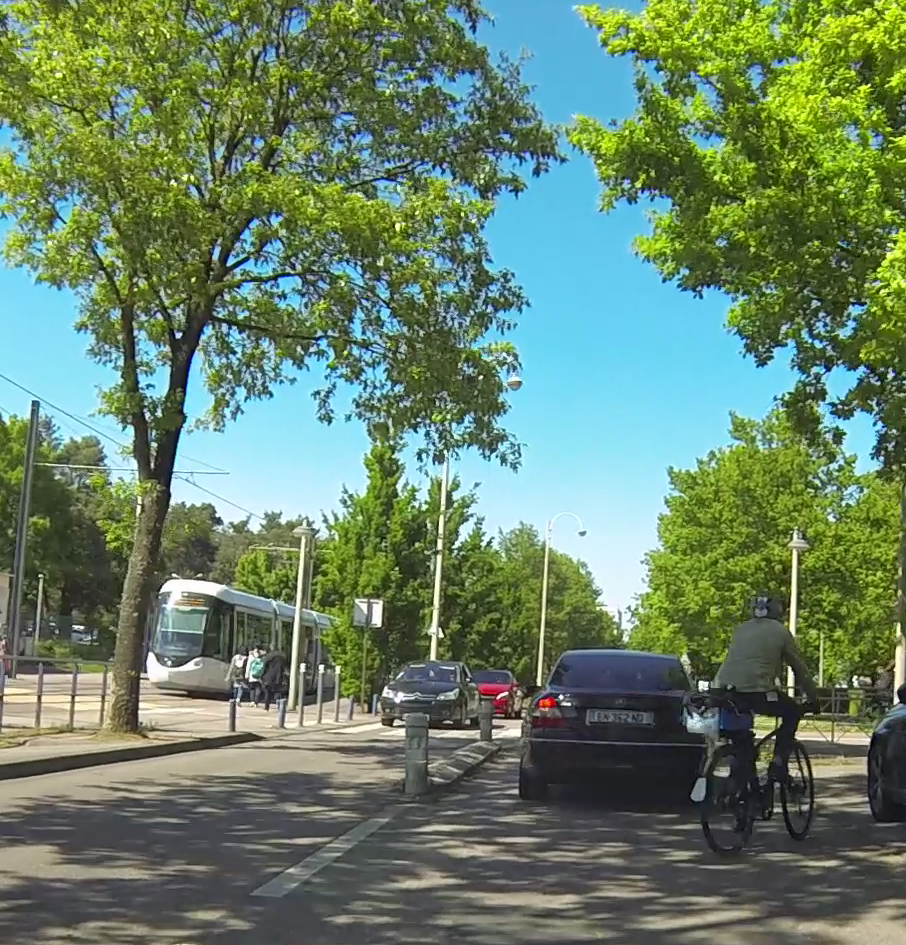
\includegraphics[width=\linewidth]{0088999.png}
	\end{subfigure}
	\caption{Examples of images in the RGB dataset.}
	\label{fig:rgb_example}
\end{figure}

Our \ac{CycleGAN}s were trained for 400 epochs on randomly cropped patches of size $200\times 200$. As for the constraints, we found experimentally that setting the hyper-parameters $\mu = 1$ and $\nu = 1$ in equation \eqref{eqn:lfinal} provides the best performances. As for the original CycleGAN, the hyper-parameter $\lambda$, controlling the reconstruction cost,
was set to $\lambda = 10$. The learning rate is decreased linearly from $2 \times 10^{-4}$ to $2 \times 10^{-6}$ during the 400 training epochs.

To evaluate the effectiveness of our trained generative model, we consider KITTI \citep{Geiger2012} and BDD100K \citep{Yu2020}(only using daytime images since polarimetry fails to characterize objects during nighttime) which often serve as test-bed in applications related to road scene object detection. The constrained-output CycleGAN we train is used to transfer RGB images from KITTI and BDD100K to the polarimetric domain. The resulting datasets are denoted respectively as Polar-KITTI and Polar-BDD100K. Since the CycleGAN architecture is fully convolutional, it has no requirement on the size of the input image. Therefore, even if the model was trained on $200 \times 200$ patches, it scales straightforwardly to the images of size $1250 \times 375$ from KITTI and of size $1280 \times 720$ from BDD100K datasets.

To assess whether or not fulfilling the physical  constraints is paramount, we investigate a variant of Polar-KITTI and Polar-BDD100K: we learn a standard unconstrained CycleGAN based on the same unpaired RGB/polarimetric images. It is worth mentioning that the so generated polarization-encoded images do not mandatory satisfy the feasibility constraints. 

\subsubsection{- Evaluation of the generated images} \label{subsec:eval_gen_img}
In order to assert the ability of the generated Polar-KITTI and Polar-BDD100K datasets to preserve the relevant features for road scene applications, we train a detection network following the setup in Figure~\ref{fig:experimental_setup}. For this experiment, a RetinaNet-50 \citep{Lin2017} pre-trained on the MS COCO dataset \citep{Lin2014} is fine-tuned in two different settings. In the first setup the detection model is fine-tuned based on the original RGB KITTI (or BDD100K) while the second experimental setting considers the fine-tuning on the generated polarimetric images from KITTI (Polar-KITTI) or BDD100K (Polar-BDD100K) datasets. Afterwards the final detection models are obtained in both settings by a final fine-tuning on the real polarimetric dataset (see Table \ref{tab:dataset_properties}). The same experiments were carried out for the unconstrained variant of the generated images.

\begin{figure}
	\centering
	\vspace{-1cm}
	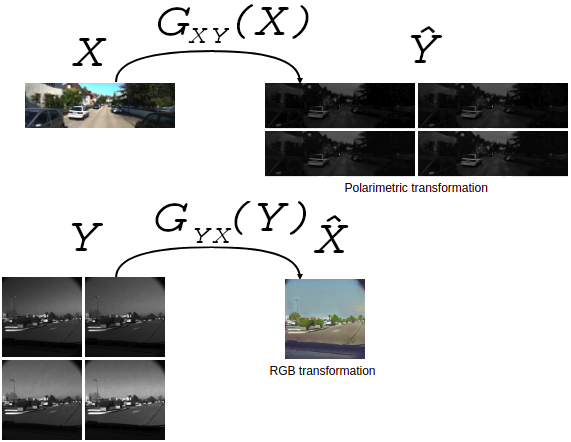
\includegraphics[width=\textwidth*4/5]{Final_experiment_correction_1.png}\\
	\hrulefill\vspace{15pt}\par
	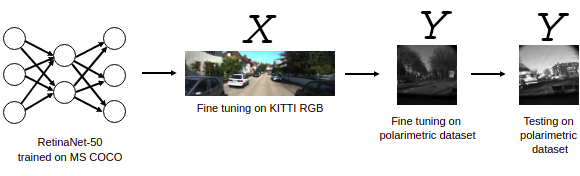
\includegraphics[width=\textwidth]{Final_experiment_correction_2.png}\\
	\hrulefill\vspace{15pt}\par
	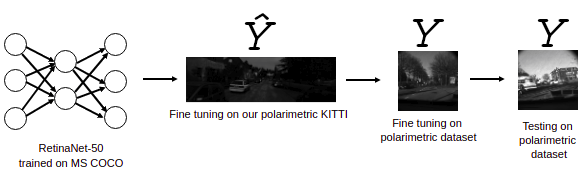
\includegraphics[width=\textwidth]{Final_experiment_correction_3.png}
	\caption[Setup of the detection evaluation experiment]{Setup of the detection evaluation experiment. The procedure is illustrated with the KITTI dataset and straightforwardly extends to the BDD100K dataset. Top: domain-transfer procedure with our model; Center: baseline setup; Bottom: our setup}
	\label{fig:experimental_setup}
\end{figure}

Overall, the trained CycleGANs and detection networks under these settings are evaluated in qualitative and quantitative ways. The end goal is to check: (i) the ability of the generated images to help learning polarimetry-based features for object detection, and (ii) the influence of respecting the polarimetric feasibility constraints on detection performances.

We  measure the visual quality of the generated images by computing the classical Fréchet Inception Distance \citep{Heusel2017} (see Section \ref{subs:evaluation_methods}). Computing this distance requires to extract visual features from each set of images (real and generated) using a pre-trained deep neural network (usually an Inception v3 \citep{Szegedy2016} network pre-trained on \ac{ImageNet} \citep{Deng2009}) and to evaluate the Fréchet (or Wasserstein) distance between the distributions of these features, which are assumed be Gaussian distributions (thoroughly explained in \citesec{subs:evaluation_methods}). We calculate this distance using 500 images from each generated polarimetric dataset and from the test set as described in Table \ref{tab:dataset_properties}.

As feature extractor, since the classical Inception v3 network is not adapted to polarimetric images, we use the convolutional part of a polarimetry-adapted RetinaNet detection network \citep{Blin2019}, which has been trained on the MS-COCO dataset and fine-tuned on a real polarimetric dataset.
%
In order to evaluate the improvements in the detection, we compute the error rate evolution $ER_o$. The improvement $ER_o$ on the detection of the object $o$ is given by:
$$
ER_o = \frac{1 - \ac{AP}_o^{p} - (1 - AP_o^{RGB})}{1-AP_o^{RGB}}\enspace,
$$

\noindent where $\ac{AP}_o^{RGB}$ and $AP_o^{p}$ respectively denote the average precision for object $o$ detection in \ac{RGB} and in polarimetric images.

\subsubsection{- Results and discussion}

\CR{Ajouter à terme les expériences avec projection} First we evaluate whether the generated images are qualitatively coherent. For the sake, we reconstruct the polarimetric images from their RGB generation, which refers to $\G_{XY} \circ \G_{YX}$ in subsection $2.2$. The reconstruction of these RGB images is shown in Figure~\ref{fig:reco_polar}. 
% A visual comparison of the same generated polarimetric image with and without constraints is illustrated in Figure~\ref{fig:generated_kitti}. As can be seen, the scene content of the generated images is preserved.
%\RB{La Figure 7 est-elle vraiment pertinente en fin de compte? Elle prend beaucoup de place et au final on ne comprend pas ce qu'elle cherche à démontrer}

\begin{figure}
	\centering
	% 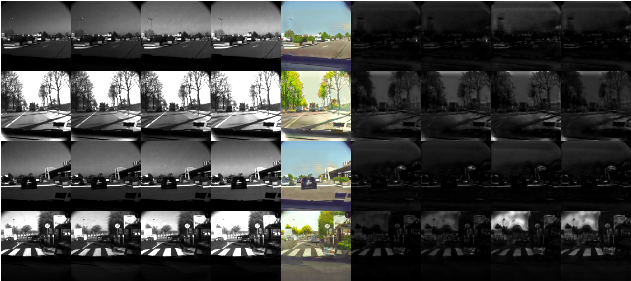
\includegraphics[width=\linewidth]{reco_polar.png}
	\begin{subfigure}{.11\textwidth}
		\centering
		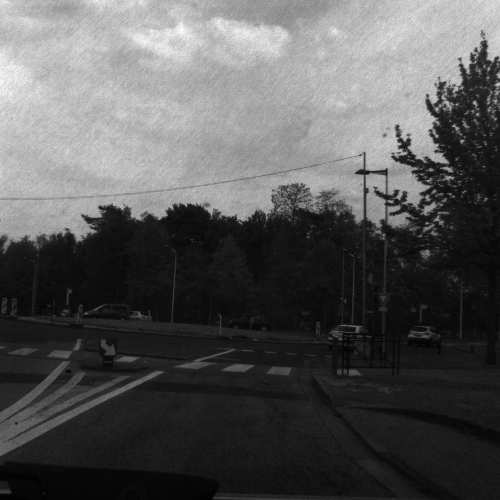
\includegraphics[width=\linewidth]{0001611_I0.png}
	\end{subfigure}%
	\begin{subfigure}{.11\textwidth}
		\centering
		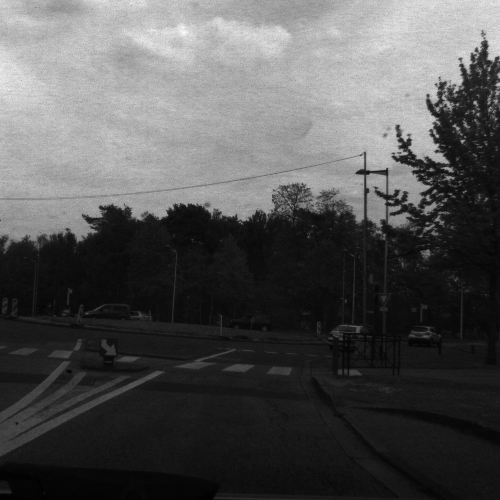
\includegraphics[width=\linewidth]{0001611_I45.png}
	\end{subfigure}%
	\begin{subfigure}{.11\textwidth}
		\centering
		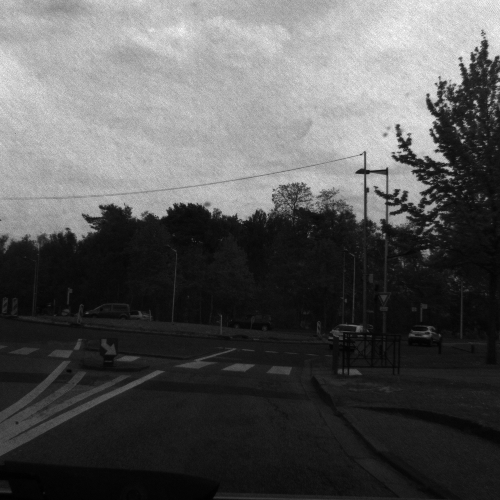
\includegraphics[width=\linewidth]{0001611_I90.png}
	\end{subfigure}%
	\begin{subfigure}{.11\textwidth}
		\centering
		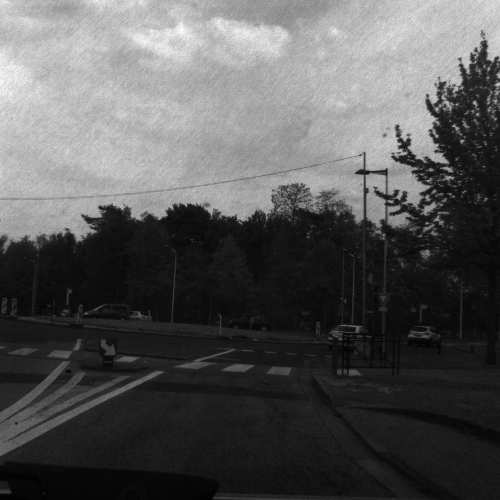
\includegraphics[width=\linewidth]{0001611_I0.png}
	\end{subfigure}%
	\begin{subfigure}{.105\textwidth}
		\centering
		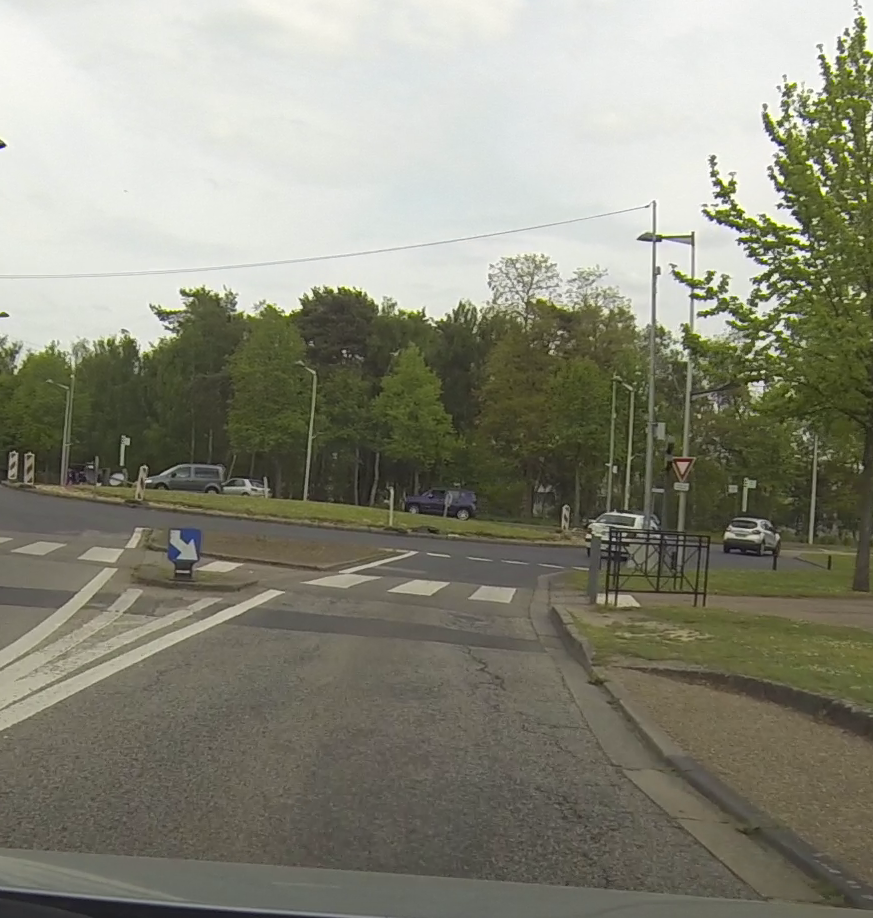
\includegraphics[width=\linewidth]{0003024.png}
	\end{subfigure}%
	\begin{subfigure}{.105\textwidth}
		\centering
		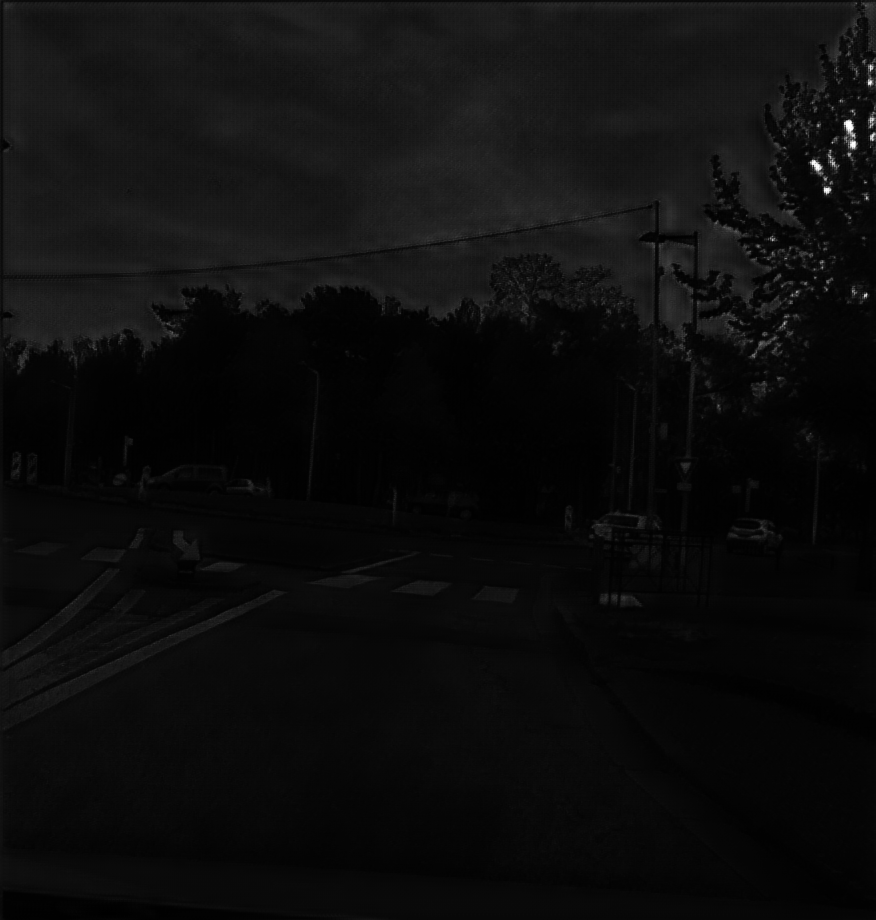
\includegraphics[width=\linewidth]{I0_0003024.png}
	\end{subfigure}%
	\begin{subfigure}{.105\textwidth}
		\centering
		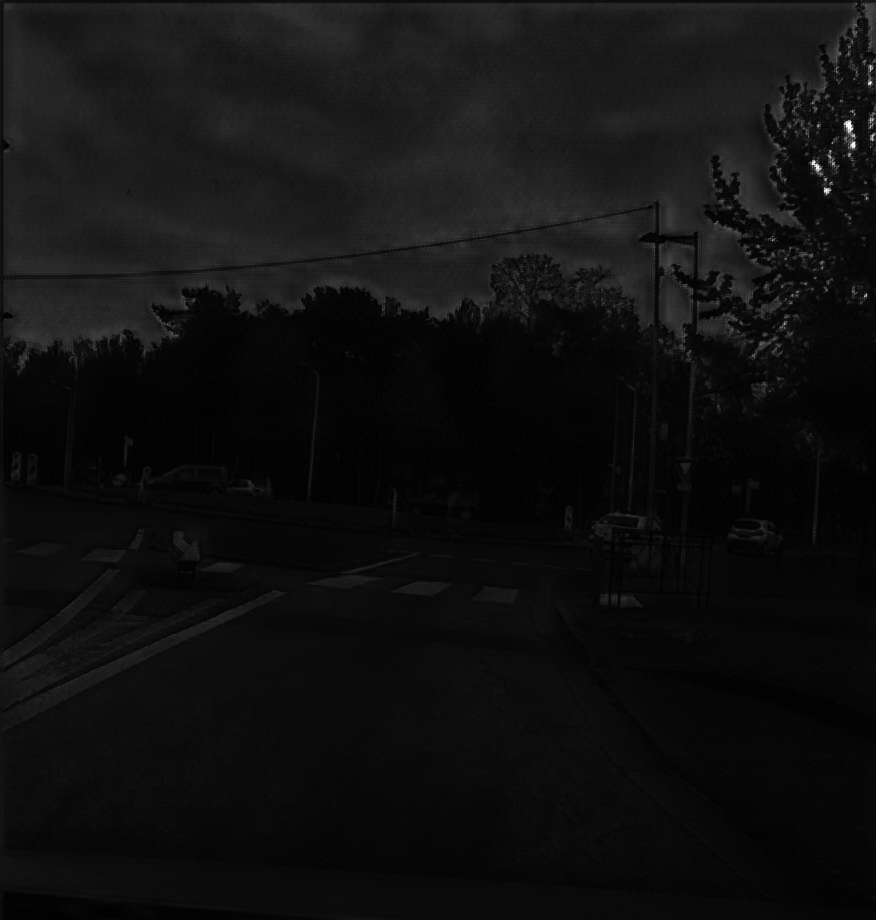
\includegraphics[width=\linewidth]{I45_0003024.png}
	\end{subfigure}%
	\begin{subfigure}{.105\textwidth}
		\centering
		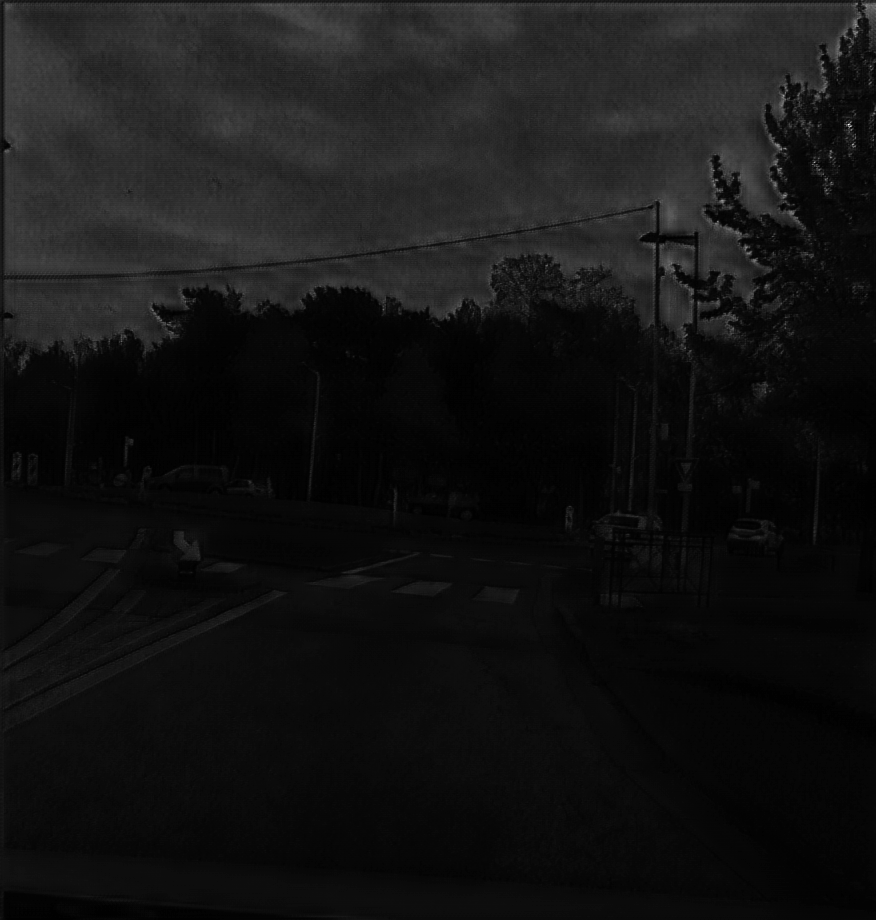
\includegraphics[width=\linewidth]{I90_0003024.png}
	\end{subfigure}%
	\begin{subfigure}{.105\textwidth}
		\centering
		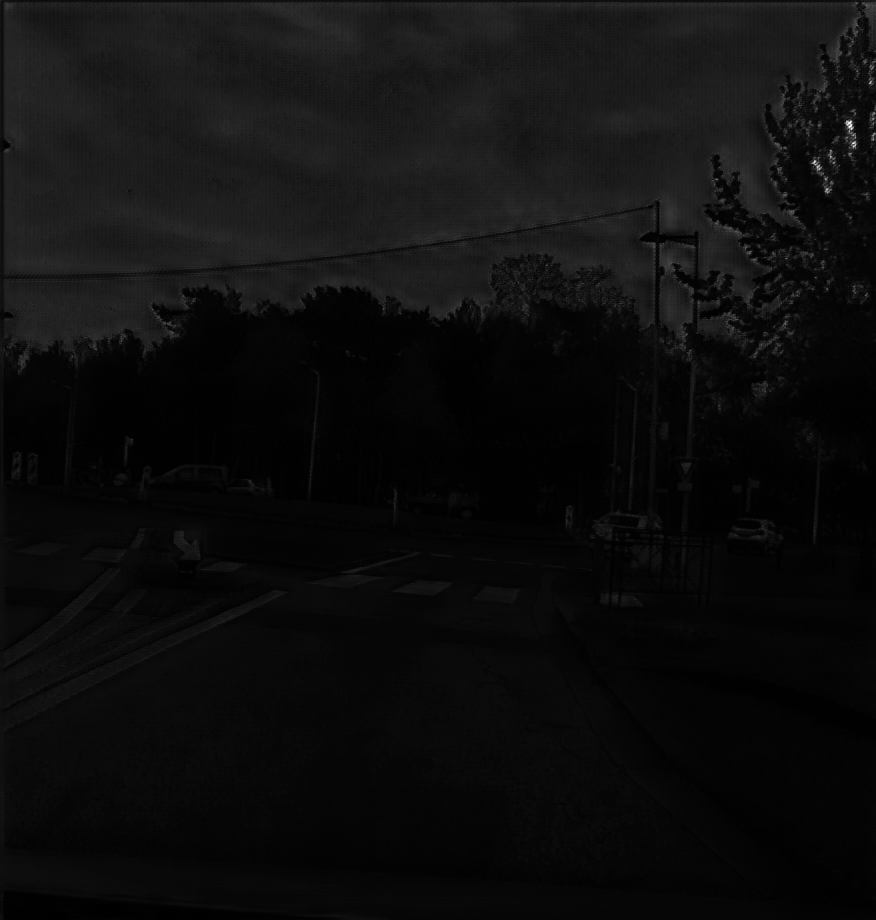
\includegraphics[width=\linewidth]{I135_0003024.png}
	\end{subfigure}
	\begin{subfigure}{.11\textwidth}
		\centering
		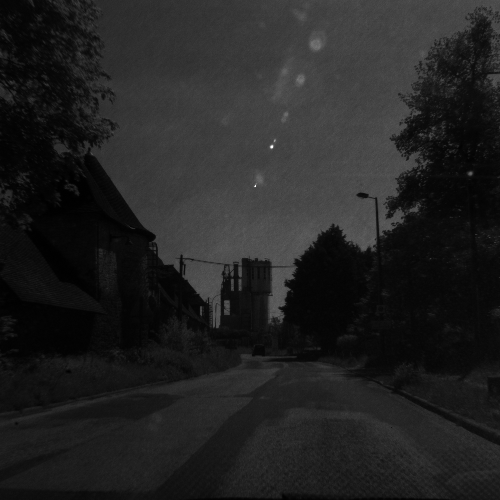
\includegraphics[width=\linewidth]{0026648_I0.png}
	\end{subfigure}%
	\begin{subfigure}{.11\textwidth}
		\centering
		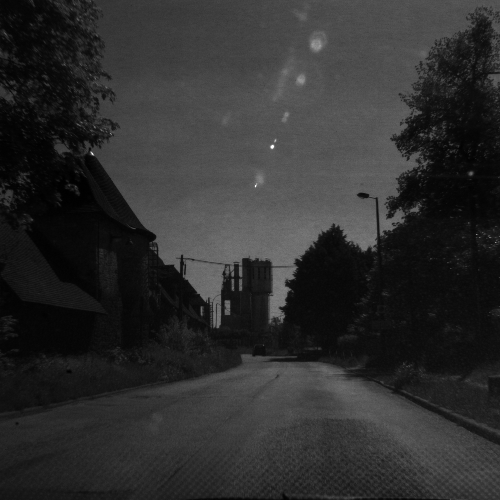
\includegraphics[width=\linewidth]{0026648_I45.png}
	\end{subfigure}%
	\begin{subfigure}{.11\textwidth}
		\centering
		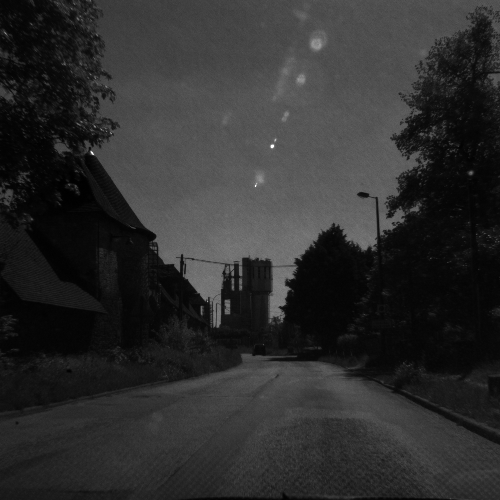
\includegraphics[width=\linewidth]{0026648_I90.png}
	\end{subfigure}%
	\begin{subfigure}{.11\textwidth}
		\centering
		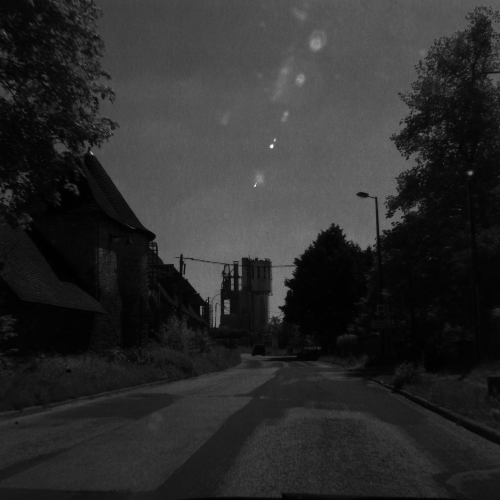
\includegraphics[width=\linewidth]{0026648_I135.png}
	\end{subfigure}%
	\begin{subfigure}{.105\textwidth}
		\centering
		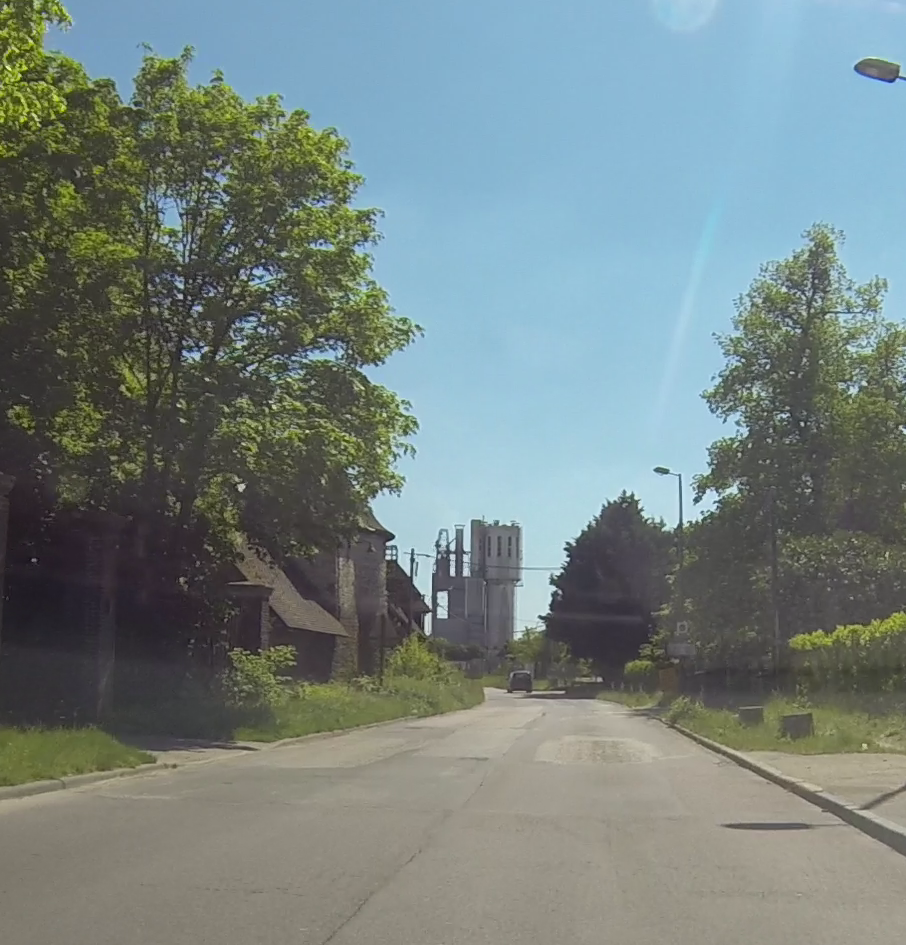
\includegraphics[width=\linewidth]{0033019.png}
	\end{subfigure}%
	\begin{subfigure}{.105\textwidth}
		\centering
		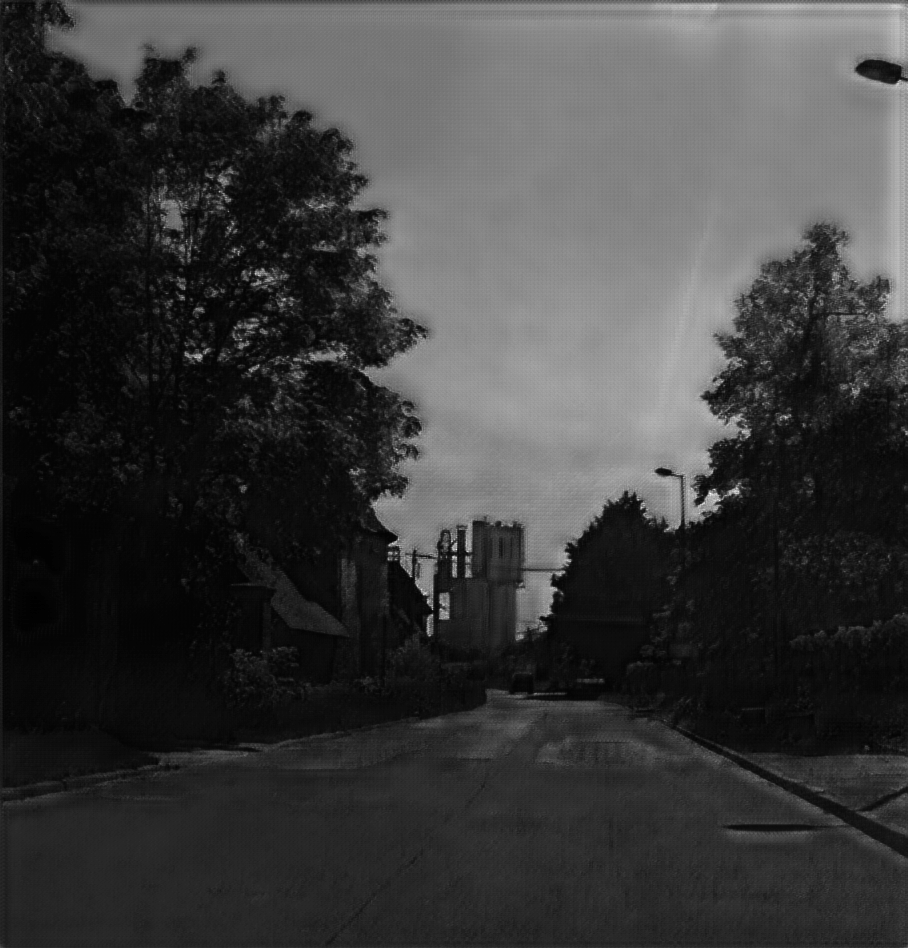
\includegraphics[width=\linewidth]{I0_0033019.png}
	\end{subfigure}%
	\begin{subfigure}{.105\textwidth}
		\centering
		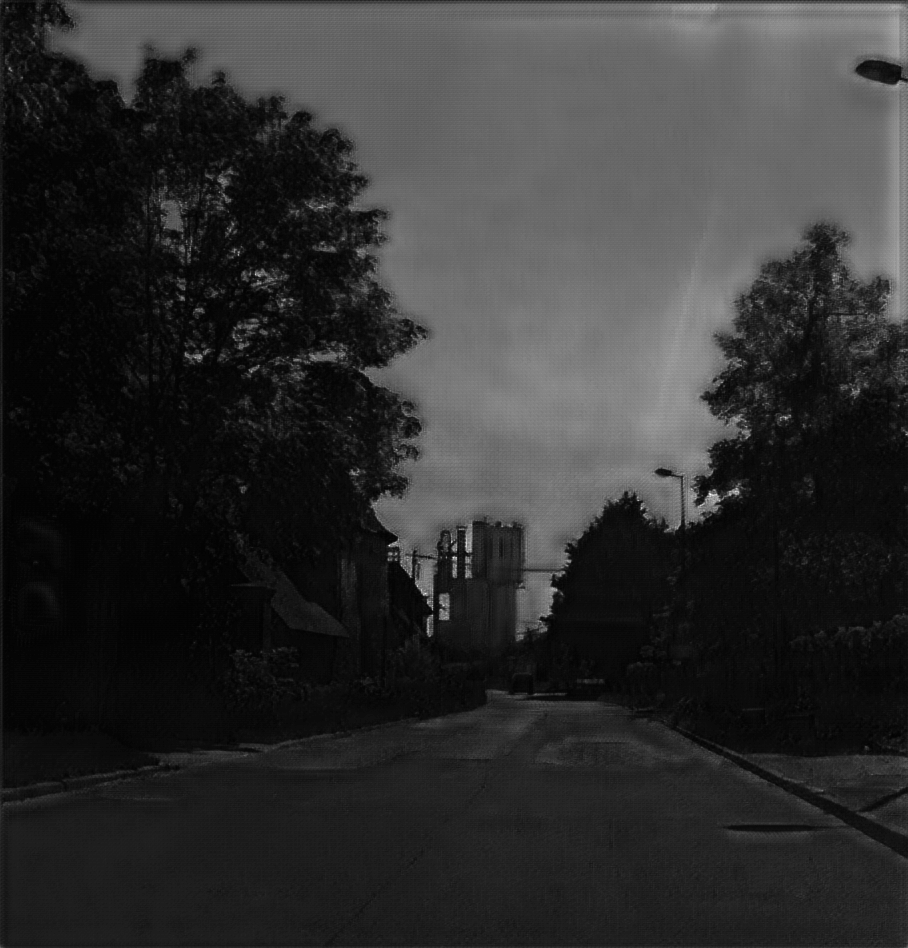
\includegraphics[width=\linewidth]{I45_0033019.png}
	\end{subfigure}%
	\begin{subfigure}{.105\textwidth}
		\centering
		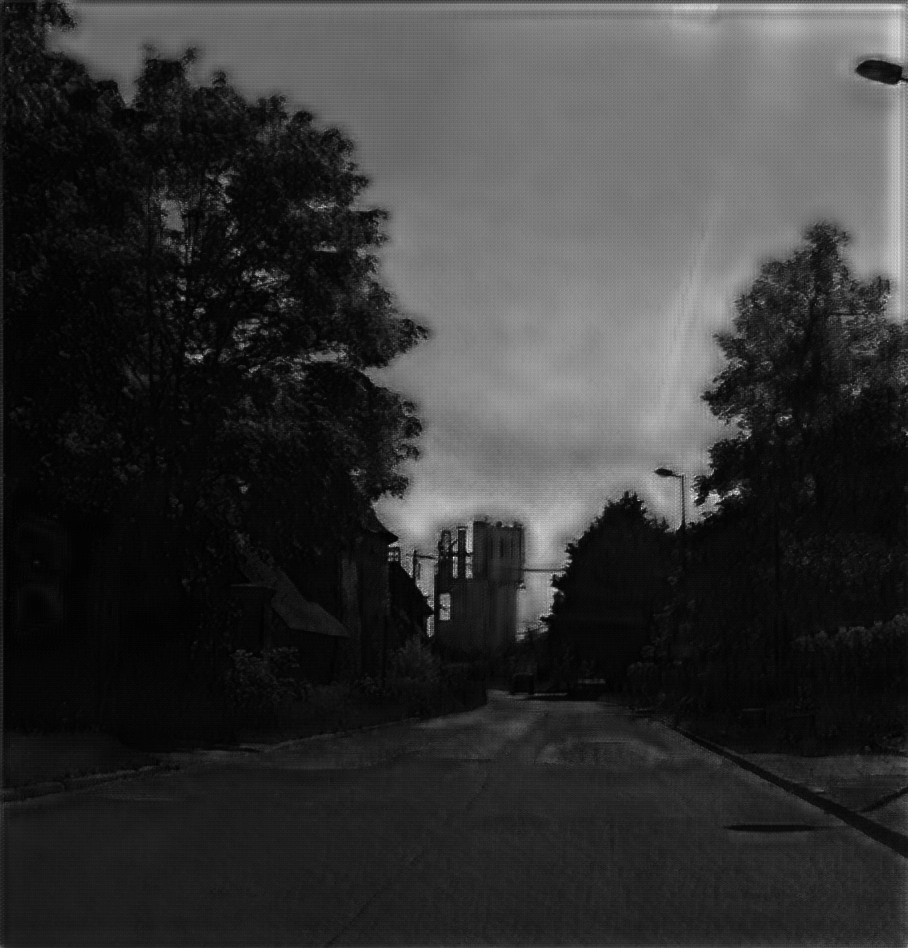
\includegraphics[width=\linewidth]{I90_0033019.png}
	\end{subfigure}%
	\begin{subfigure}{.105\textwidth}
		\centering
		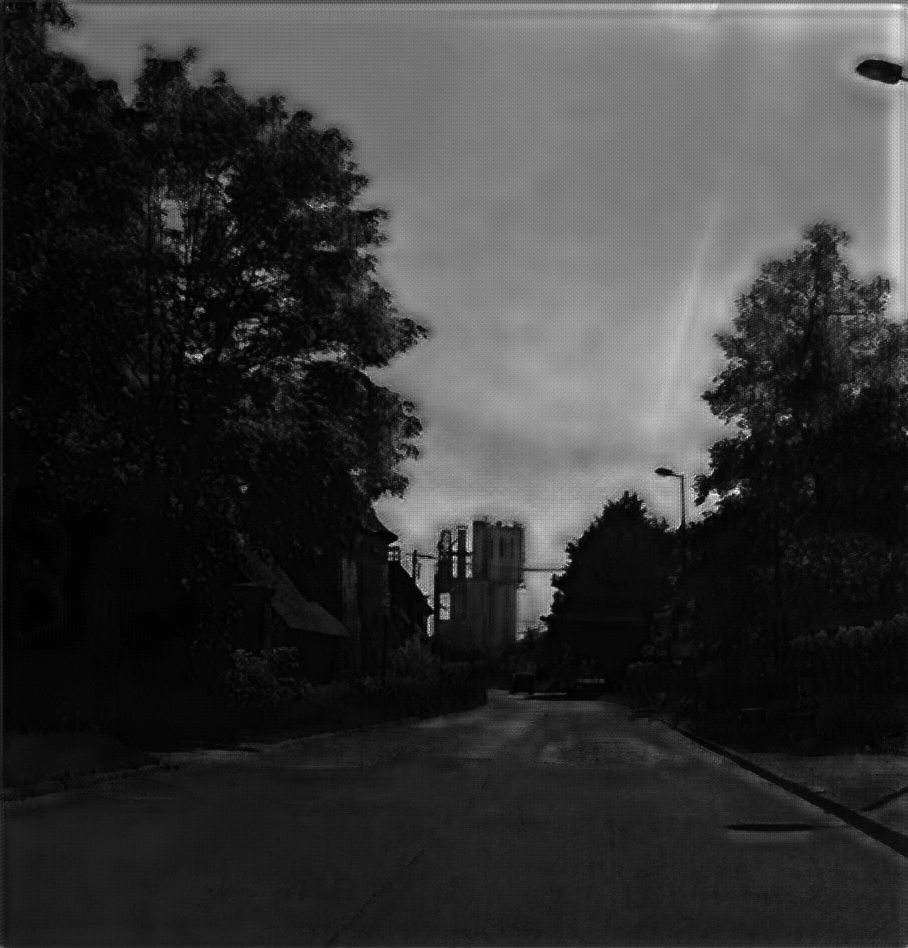
\includegraphics[width=\linewidth]{I135_0033019.png}
	\end{subfigure}
	\begin{subfigure}{.11\textwidth}
		\centering
		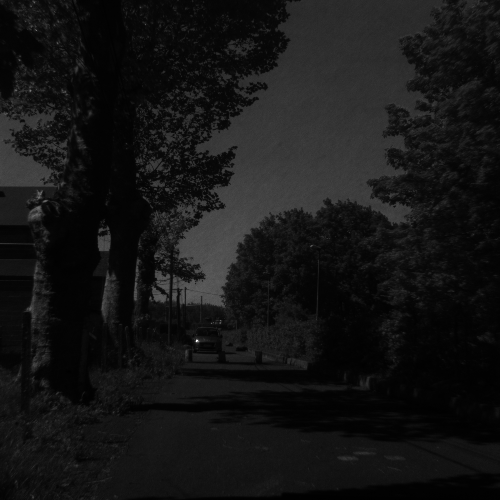
\includegraphics[width=\linewidth]{0033248_I0.png}
	\end{subfigure}%
	\begin{subfigure}{.11\textwidth}
		\centering
		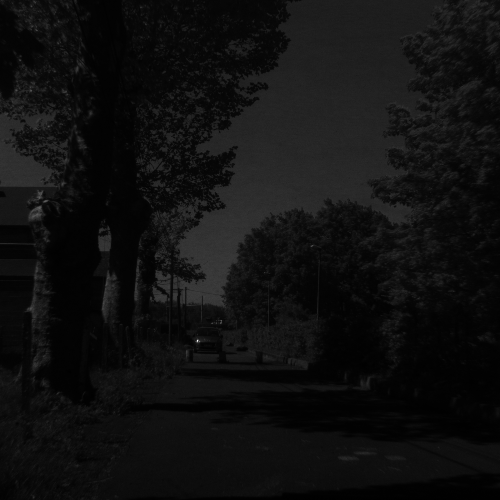
\includegraphics[width=\linewidth]{0033248_I45.png}
	\end{subfigure}%
	\begin{subfigure}{.11\textwidth}
		\centering
		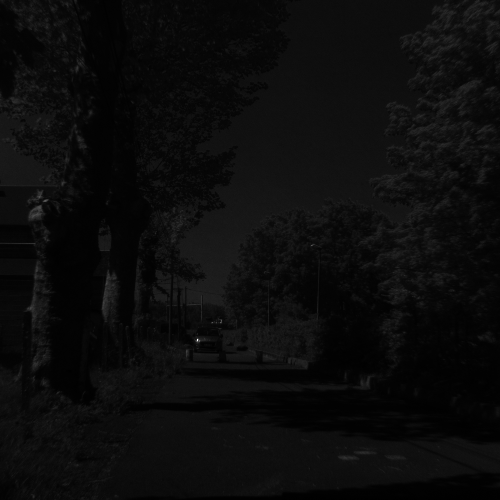
\includegraphics[width=\linewidth]{0033248_I90.png}
	\end{subfigure}%
	\begin{subfigure}{.11\textwidth}
		\centering
		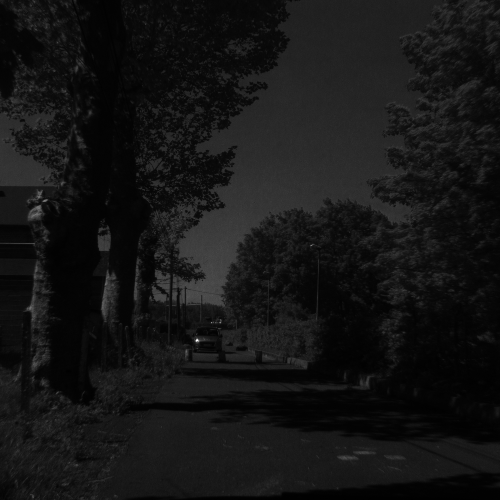
\includegraphics[width=\linewidth]{0033248_I135.png}
	\end{subfigure}%
	\begin{subfigure}{.105\textwidth}
		\centering
		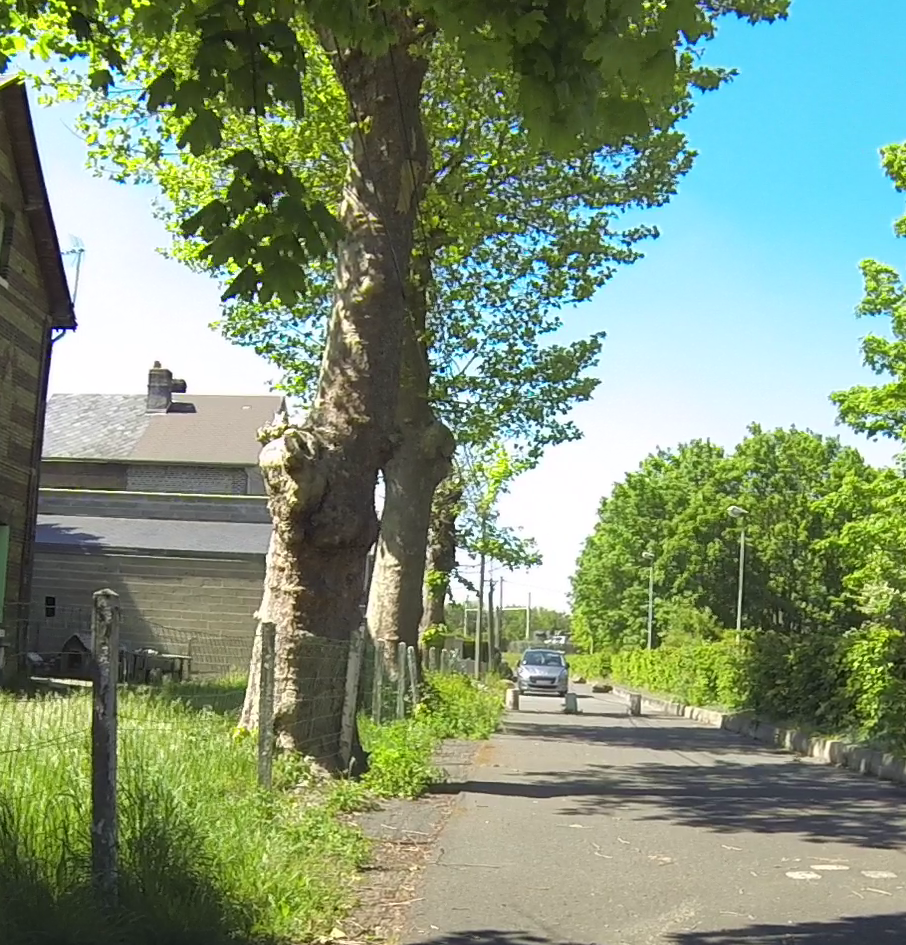
\includegraphics[width=\linewidth]{0040999.png}
	\end{subfigure}%
	\begin{subfigure}{.105\textwidth}
		\centering
		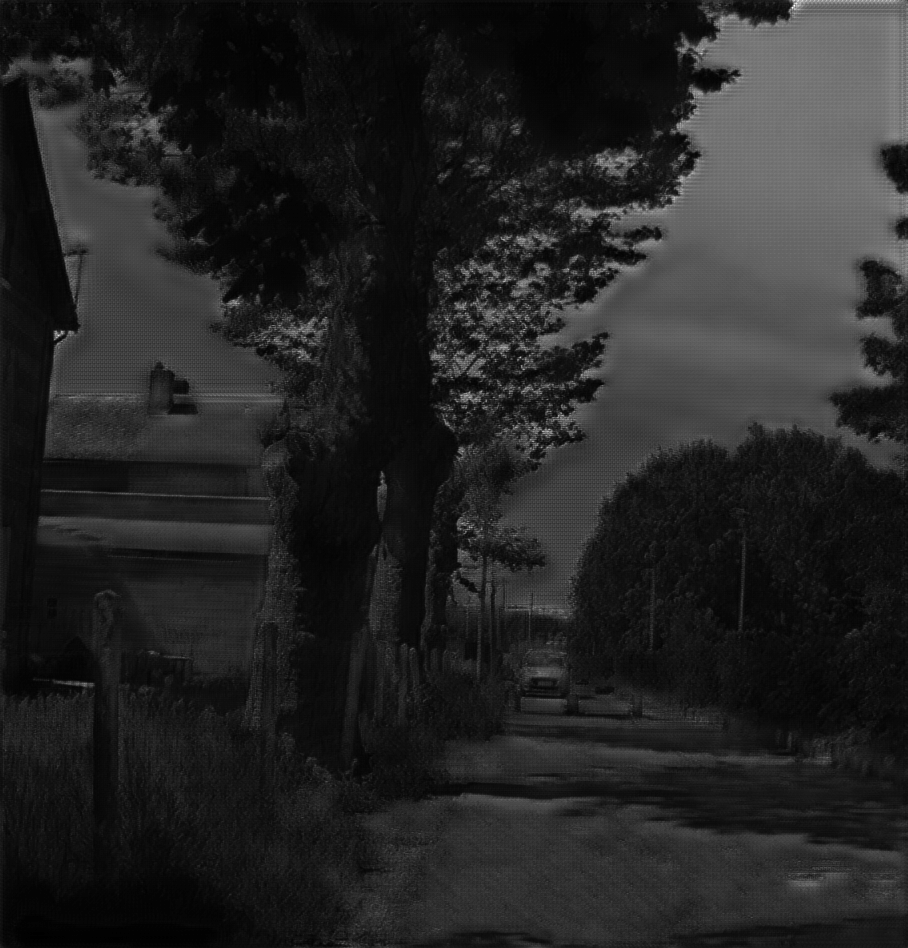
\includegraphics[width=\linewidth]{I0_0040999.png}
	\end{subfigure}%
	\begin{subfigure}{.105\textwidth}
		\centering
		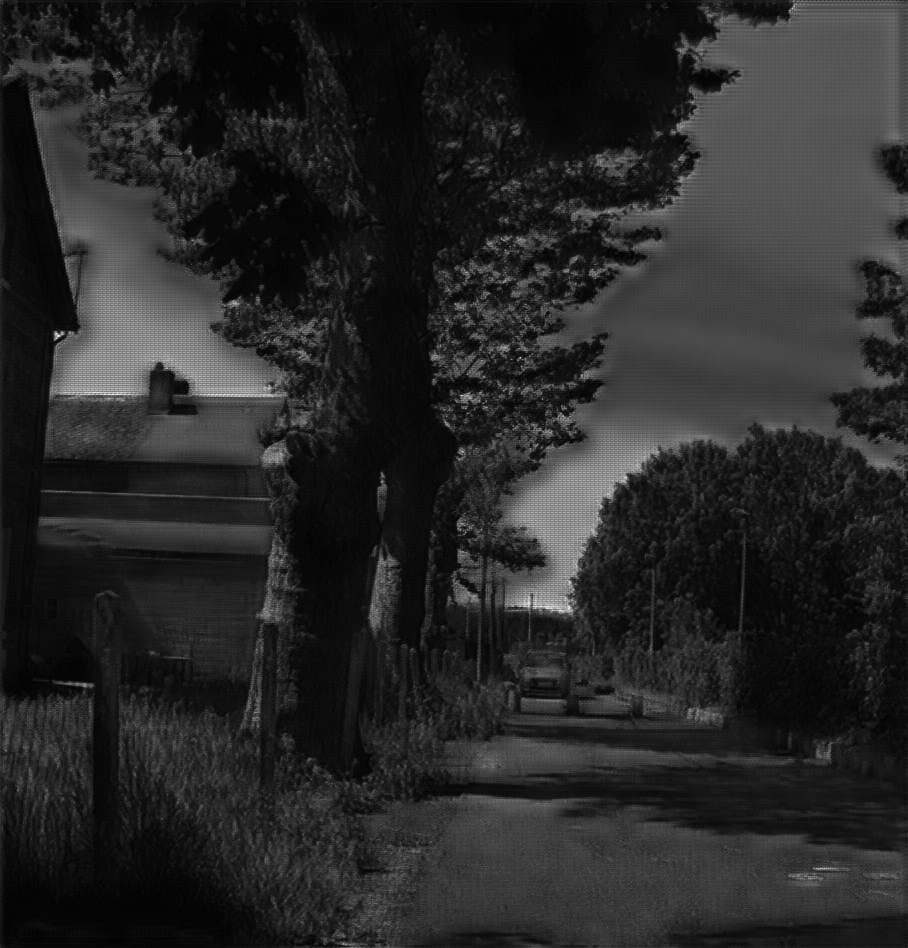
\includegraphics[width=\linewidth]{I45_0040999.png}
	\end{subfigure}%
	\begin{subfigure}{.105\textwidth}
		\centering
		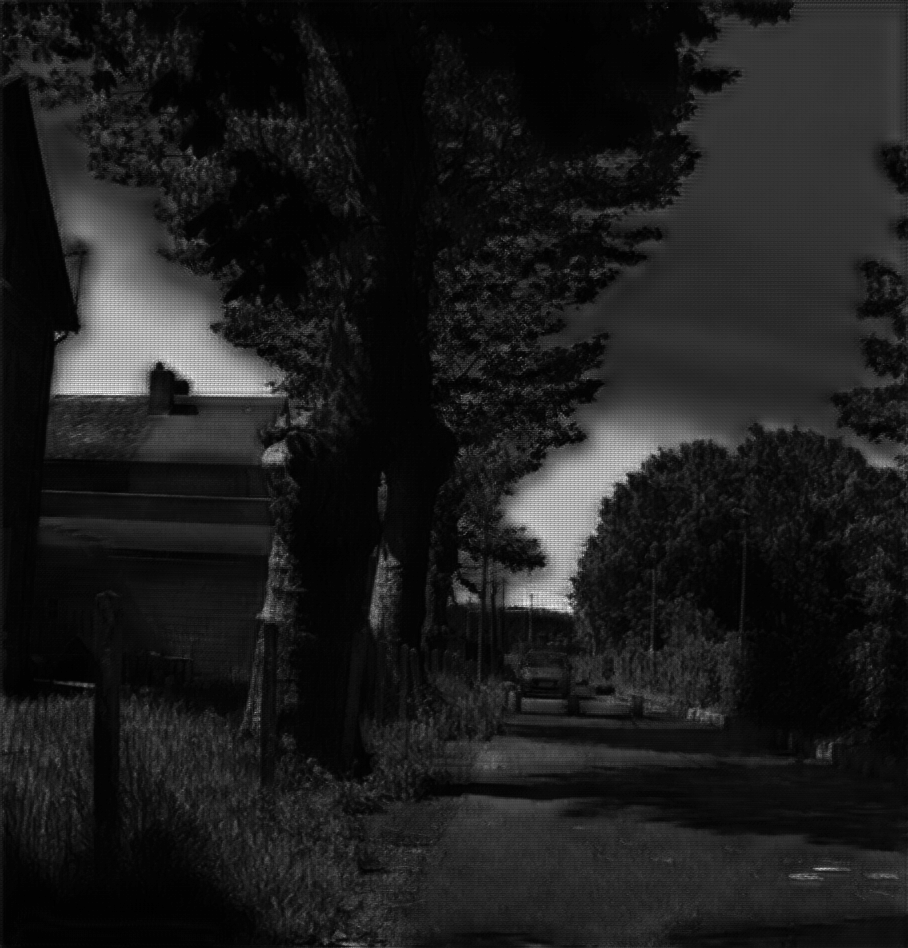
\includegraphics[width=\linewidth]{I90_0040999.png}
	\end{subfigure}%
	\begin{subfigure}{.105\textwidth}
		\centering
		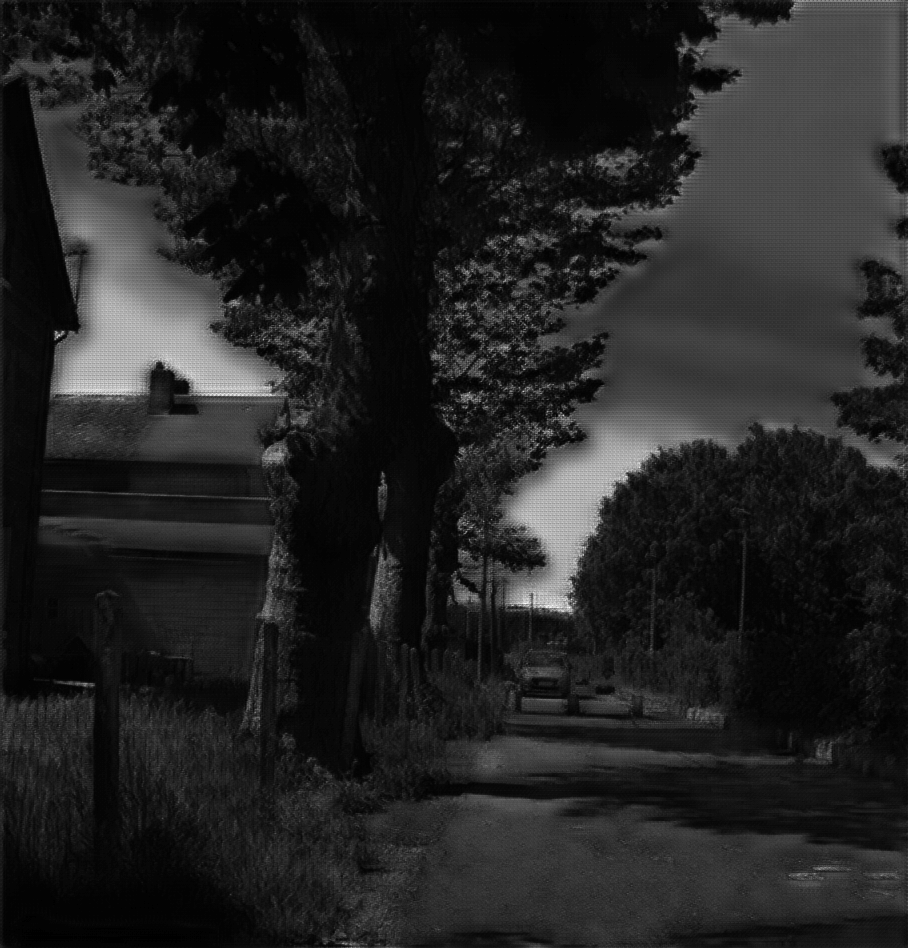
\includegraphics[width=\linewidth]{I135_0040999.png}
	\end{subfigure}
	\begin{subfigure}{.11\textwidth}
		\centering
		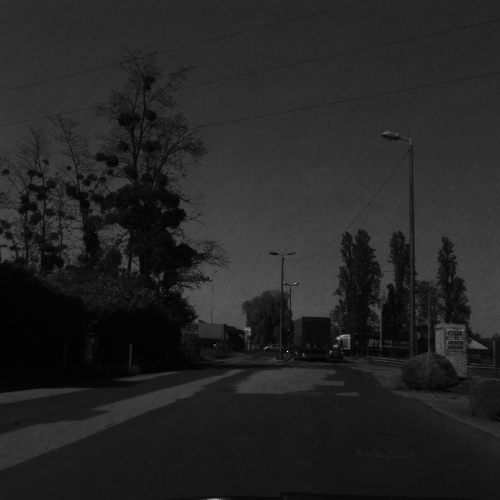
\includegraphics[width=\linewidth]{0048448_I0.png}
	\end{subfigure}%
	\begin{subfigure}{.11\textwidth}
		\centering
		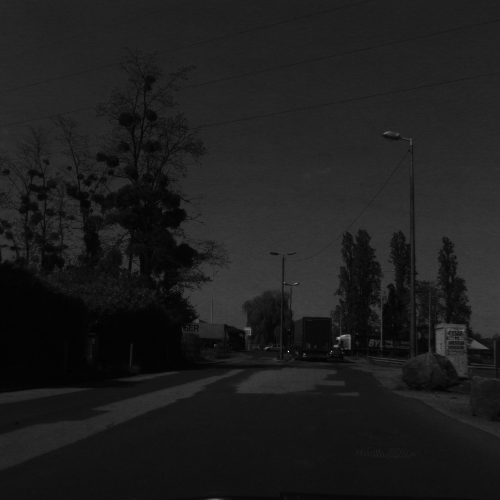
\includegraphics[width=\linewidth]{0048448_I45.png}
	\end{subfigure}%
	\begin{subfigure}{.11\textwidth}
		\centering
		\includegraphics[width=\linewidth]{0048448_I90.png}
	\end{subfigure}%
	\begin{subfigure}{.11\textwidth}
		\centering
		\includegraphics[width=\linewidth]{0048448_I135.png}
	\end{subfigure}%
	\begin{subfigure}{.105\textwidth}
		\centering
		\includegraphics[width=\linewidth]{0059179.png}
	\end{subfigure}%
	\begin{subfigure}{.105\textwidth}
		\centering
		\includegraphics[width=\linewidth]{I0_0059179.png}
	\end{subfigure}%
	\begin{subfigure}{.105\textwidth}
		\centering
		\includegraphics[width=\linewidth]{I45_0059179.png}
	\end{subfigure}%
	\begin{subfigure}{.105\textwidth}
		\centering
		\includegraphics[width=\linewidth]{I90_0059179.png}
	\end{subfigure}%
	\begin{subfigure}{.105\textwidth}
		\centering
		\includegraphics[width=\linewidth]{I135_0059179.png}
	\end{subfigure}
	\caption[Examples  of polarimetric image reconstruction]{Examples  of polarimetric image reconstruction. From left to right: $I_0$, $I_{45}$, $I_{90}$ and $I_{135}$ ground truth, RGB image and $I_0$, $I_{45}$, $I_{90}$ and $I_{135}$ generated from RGB image.}
	\label{fig:reco_polar}
\end{figure}

% \begin{figure}
%     \centering
%     \includegraphics[width=\linewidth]{comparison_generation.png}
%     \caption{Example of generated images (Polar-KITTI). The left column represents the generation with constraints and the right column refers to image generation without constraints. From top to bottom: $I_0$, $I_{45}$, $I_{90}$ and $I_{135}$.}
%     \label{fig:generated_kitti}
% \end{figure}

As for the constraints, Table \ref{tab:polar_constraints} shows how including them to the \ac{CycleGAN}'s loss helps generating images which better fulfill the physical polarimetric properties at the pixel scale. The errors related to the constraints $\mathcal{C}_1$ and $\mathcal{C}_2$ on generated images using our approach are consistent with the observed errors on the real images, whereas the unconstrained approach yields poor results. Obviously, constraint $\mathcal{C}_3$ is met for all generated images thanks to the $\tanh$ activation at the last layer of the generative models. Additionally, the obtained Fréchet Inception Distances (see table \ref{tab:polar_constraints}) indicates that taking the constraints into account improves visual and physical quality of the generated samples.


\begin{table}
	\begin{center}
		\begin{tabular}{c c c c || c}
			\Bigrule
			Datasets & $\mathcal{C}$ & Mean & Median & FID \\
			\Bigrule
			Real & $\mathcal{C}_1$ & 0.06 $\pm$ 0.04 & 0.04  \\
			polar & $\mathcal{C}_2$ & 2.47 $\pm$ 7.11\% & 0.48\% & N/A \\
			& $\mathcal{C}_3$ & 0\% & 0\% \\
			\bigrule 
			Generated & $\mathcal{C}_1$ & 0.26 $\pm$ 0.19 & 0.23 \\
			polar no $\mathcal{C}$ & $\mathcal{C}_2$ & 27.31 $\pm$ 43.5\% & 2.15\% & 6022.7\\
			& $\mathcal{C}_3$ & 0\% & 0\% \\
			\bigrule 
			Relaxed & $\mathcal{C}_1$ & 0.12 $\pm$ 0.04 & 0.12 \\
			constraints  & $\mathcal{C}_2$ & 1.55 $\pm$ 3.36\% & 0.14\% &\textbf{4485.1}\\
			& $\mathcal{C}_3$ & 0\% & 0\% \\
			\bigrule 
			Projection to & $\mathcal{C}_1$ & 0 $\pm$ 0 & 0\\
			the constraints  & $\mathcal{C}_2$ & 0 $\pm$ 0\% & 0\% & TODO \\
			& $\mathcal{C}_3$ & 0\% & 0\% \\
			\bigrule 
			Learned with & $\mathcal{C}_1$ & 0 $\pm$ 0 & 0\\
			proximal & $\mathcal{C}_2$ & 0 $\pm$ 0\% & 0\% & TODO\\
			& $\mathcal{C}_3$ & 0\% & 0\% \\
		\end{tabular}
		\caption[Evaluation of the generated images]{Evaluation of the constraint fulfillment using the designed losses $L_{\mathcal{C}_1}$ and $L_{\mathcal{C}_2}$ at the pixel scale, and  the visual quality using the Fréchet Inception Distance (\ac{FID})\footnote{Note that the scale of the \ac{FID} scores computed with the pre-trained RetinaNet is larger than when using a pre-trained Inception v3 network.}. Here, the column $\mathcal{C}$ indicates the evaluated constraint. $\mathcal{C}_1$ refers to the constraints $\vy = \ma\ma^\dagger\vy$, $\mathcal{C}_2$ to $\vs_0^2 \geqslant \vs_1^2 + \vs_2^2$ and $\mathcal{C}_3$ to $\vs_0 > 0$. The mean and the median of the percentage of pixels in an image that do not fulfill the constraints $\mathcal{C}_2$ and $\mathcal{C}_3$ are computed. Regarding the constraint $\mathcal{C}_1$, we compute the mean and the median of $||\vy - \ma\ma^\dagger\vy|| / (||\vy|| + ||\ma\ma^\dagger\vy||)$.}
		\label{tab:polar_constraints}
	\end{center}
\end{table}

Next, we show the benefit of the generated images in object detection task, enabling to verify that objects in them are globally physically coherent. 
The RetinaNet-based detection model were trained according to the setups described in Section \ref{subsec:eval_gen_img} and the obtained detection performances in term of mean average precision ($\ac{mAP}$) are summarized in Table \ref{tab:obtained_results}. We choose not to evaluate the bike and motorbike detection performances as the polarimetric dataset does not contain enough objects of those two classes.

\begin{table}
	\begin{center}
		\begin{tabular}{c c c c| c c cc}
			\Bigrule
			Databases used & Class & Test & $ER_o$ & Databases used & Class & Test & $ER_o$ \\
			\Bigrule
			KITTI RGB & person & 0.663 & N/A & BDD100K RGB & person & 0.736 & N/A \\
			+ real polar & car & 0.785 & N/A & + real polar & car & \textbf{0.821} & N/A \\
			\multicolumn{2}{c}{$mAP$} & 0.724 & N/A & \multicolumn{2}{c}{$mAP$} & 0.778 & N/A \\
			\bigrule 
			Polar-KITTI  & person & 0.673 & -0.03 & Polar-BDD100K  & person & 0.720 & 0.06 \\
			no $\mathcal{C}$ + real polar & car & 0.786 & -0.01 & no $\mathcal{C}$ + real polar & car & 0.816 & 0.03 \\
			\multicolumn{2}{c}{$mAP$} & 0.730 & -0.02 & \multicolumn{2}{c}{$mAP$} & 0.768 & 0.05 \\
			\bigrule 
			Polar-KITTI with  & person & \textbf{0.704} & -0.12 & Polar-BDD100K  & person & \textbf{0.762} & -0.10 \\
			relaxed $\mathcal{C}$  & car & \textbf{0.794} & -0.04 & with relaxed $\mathcal{C}$ & car & 0.815 & 0.03 \\
			\multicolumn{2}{c}{$mAP$} & \textbf{0.749} & -0.09 & \multicolumn{2}{c}{$mAP$} & \textbf{0.789} & -0.05 \\
			\bigrule 
			Polar-KITTI with  & person & 0 & 0 & Polar-BDD100K  & person & 0 & 0 \\
			projection on $\mathcal{C}$ & car & 0 &0 & with projection $\mathcal{C}$ & car & 0 & 0 \\
			\multicolumn{2}{c}{$mAP$} & 0 & 0 & \multicolumn{2}{c}{$mAP$} & 0 & 0 \\
			\bigrule 
			Polar-KITTI with  & person & 0 & 0 & Polar-BDD100K  & person & 0 & 0 \\
			learned proximal & car &0  & 0 & with projection $\mathcal{C}$ & car & 0 & 0 \\
			\multicolumn{2}{c}{$mAP$} & 0 & 0 & \multicolumn{2}{c}{$mAP$} & 0 &0 \\
		\end{tabular}
	\end{center}
	\caption[Comparison of the detection performance after successive fine-tunings]{
	\CR{	Comparison of the detection performance after the two successive fine-tunings. RetinaNet-50 pre-trained on MS COCO is the baseline of all the experiments. The first row refers to the RetinaNet-50 fine-tuned on KITTI or BDD100K RGB. The second row refers to the fine-tuning on Polar-KITTI or Polar-BDD100K without constraints while the bottom row represents the detection models fine-tuned on Polar-KITTI or Polar-BDD100K with the constraints. All these models are finally fine-tuned on the real polarimetric dataset. }
	}
	\label{tab:obtained_results}
\end{table}

As we can see in Table \ref{tab:obtained_results}, using the generated polarimetric images improves the detection performance in real polarimetric images. The improvement is substantial for car and pedestrian detection. We achieve an improvement of 4\% for car detection and of 12\% for pedestrian detection which leads to a global improvement of 9\% in the detection, using Polar-KITTI with constraints. Similarly for Polar-BDD100K dataset, we notice an improvement of 10\% for pedestrian detection which leads to an increased $\ac{mAP}$ of 5\% (pedestrians and cars). However, we notice that for BDD100K similar detection performances are obtained either for RGB or polarimetric images and this is due to the fact that generated images using CycleGANs don't perform well on small objects. To verify that, we compared the evolution of the detections scores while setting a minimal area to the bounding boxes to be detected. The results of this experiment are shown for the training including the Polar-BDD100K and the RGB BDD100K in Figure~\ref{fig:bounding_boxes}.

\begin{figure}
	\centering
	\includegraphics[width=\linewidth]{area_bounding_boxes_study.png}
	\caption[Evolution of the average precision when setting a minimal area of the bounding boxes]{Evolution of the average precision when setting a minimal area of the bounding boxes to be detected. Here green lines refer to the evolution of cars' detection, blue lines to the evolution of the $\ac{mAP}$ and red lines to the evolution of person's detection. The dashed lines refer to the training including the BDD100K RGB and the solid lines to the training including Polar-BDD100K.}
	\label{fig:bounding_boxes}
\end{figure}

The results of this experiment showed that when the minimal area of bounding boxes increases the $\ac{AP}$ of car regarding the training including Polar-BDD100K overcomes the one including RGB BDD100K. We can thus conclude that the limit of this work is the low quality of the small objects in the generated images. 

\section{Conclusion and perspective}

In this work, we proposed an efficient way to generate realistic polarimetric images subject to physical admissibility constraints. An adapted \ac{CycleGAN} is used to achieve the generation of pixel-wise physical images. To train the proposed output-constrained CycleGAN, we combined the standard \ac{CycleGAN}'s objective function with two designed cost functions in order to handle the feasibility constraints related to each polarization-encoded pixel in the image. 
With the proposed generative model, we successfully translated RGB images from road scenes to polarimetric images showing an enhancement of the detection performances.
Future work would consist in improving the quality of the small objects in generated images. It would also be interesting to extend the generation of polarimetric images to other domains such as medical and Synthetic-Aperture Radar \CR{REF} imaging. Extension of the generation procedure to road scene images under adverse weather conditions may help improving object detection in these situations.